\documentclass[xcolor=svgnames, 10pt]{beamer}

\usepackage[utf8]{inputenc}
\usepackage[T1]{fontenc}
\usepackage[english]{babel}

%\usepackage{verbatim}

\usepackage[export]{adjustbox}

\usepackage{
    amsmath,
    amsfonts,
    etex,
    fancyvrb,
    graphicx,
    multicol,
    pifont,
    setspace,
    soul,
    spverbatim,
    textcomp,
    xcolor,
    xspace
}

\usepackage{tikz}
\usetikzlibrary{shadows}

%%%SETUP%%%
\hypersetup{
     colorlinks = true,
     linkcolor = blue,
     anchorcolor = blue,
     citecolor = blue,
     filecolor = blue,
     urlcolor = blue
     }
     
%%%THEOREMS%%%
\theoremstyle{example}
\newtheorem*{exercise}{Exercise}
\newtheorem*{question}{Question}
\newtheorem*{answer}{\emph{Answer}}
\newtheorem*{notation}{Notation}

%%%TWEAKS%%%
\setlength\arraycolsep{4pt}
\addtolength\fboxsep{10pt}
\setstretch{1.4}
\setbeamersize{description width=3em}
\setbeamersize{text margin left=.5cm,text margin right=.5cm} 
\renewcommand{\emph}{\alert}
\renewcommand{\arraystretch}{1.2}
\renewcommand{\tabcolsep}{4pt}
\setbeamercolor{alerted text}{fg=magenta}


\graphicspath{{img/}}

%for straight quotes in verbatim:
\usepackage{upquote,textcomp}

%turn off navigation symbols
\beamertemplatenavigationsymbolsempty
\setbeamertemplate{footline}[frame number]

%title page

\author
  [Dr.\ Irene Vrbik]
  {Dr.\ Irene Vrbik}

\date
  {}

\institute
  {University of British Columbia Okanagan \newline \texttt{irene.vrbik@ubc.ca}}
  
\definecolor{iyellow}{RGB}{255, 162, 23}
\definecolor{sgreen}{RGB}{118, 191, 138}

\newcommand{\yellow}[1]{\textcolor{iyellow}{#1}}
\newcommand{\red}[1]{\textcolor{red}{#1}}
\newcommand{\green}[1]{\textcolor{ForestGreen}{#1}}
\newcommand{\blue}[1]{{\textcolor{blue}{#1}}}
\newcommand{\orange}[1]{{\textcolor{orange}{#1}}}
\newcommand{\bblue}[1]{\textcolor{SteelBlue!90!gray}{#1}} % beamer blue
\newcommand{\purple}[1]{{\textcolor{purple}{#1}}}

\newcommand{\el}{\\[1em]\pause}
\newcommand{\nl}{\\[1em]}
\newcommand{\define}[1]{\textbf{\textcolor{orange}{#1}}}

%\newcommand{\answer}[1]{\textit{\textbf{\textcolor{iyellow}{#1}}}}

\newcommand{\command}[1]{\texttt{\textbf{\textcolor{DarkMagenta}{#1}}}}
\newcommand{\ipic}[2]{\includegraphics[width={#2}\textwidth]{#1}}
\newcommand{\cell}[1]{{\sf \textbf{\textcolor{DarkMagenta}{#1}}}}
\newcommand{\ra}{$\rightarrow$}

\newcommand{\ft}[1]{\frametitle{#1}}


\newenvironment{allintypewriter}{\ttfamily}{\par}
\newcommand{\bs}{$\backslash$}

\newcommand*\keystroke[1]{%
  \tikz[baseline=(key.base)]
    \node[%
      draw,
      fill=white,
      drop shadow={shadow xshift=0.25ex,shadow yshift=-0.25ex,fill=black,opacity=0.75},
      rectangle,
      rounded corners=2pt,
      inner sep=1pt,
      line width=0.5pt,
      font=\scriptsize\sffamily
    ](key) {#1\strut}
  ;
}

% timed answer
\newcommand{\tans}[2]{\textbf<#1>{\textit<#1>{{\color<#1>{iyellow}{#2}}}}}


\makeatletter
\g@addto@macro\normalsize{%
  \setlength\abovedisplayskip{0.4em}
  \setlength\belowdisplayskip{0.4em}
  \setlength\abovedisplayshortskip{0.2em}
  \setlength\belowdisplayshortskip{0.2em}
}
\makeatother


\newcommand{\cmark}{{\Large\color{green}\ding{51}}}%
\newcommand{\xmark}{{\Large\color{red}\ding{55}}}%

\newcommand{\pcmark}{\onslide<+->{\cmark}}
\newcommand{\pxmark}{\onslide<+->{\xmark}}

\newcommand{\by}{\overline{y}}
\newcommand{\ty}{\tilde{y}}

\title
  [R]
  {Introduction to Data Analytics:}
\subtitle{\Large R}
  
  \usepackage{xspace}
\newcommand{\R}{{\tt R }}

\makeatletter
\def\maxwidth{ %
  \ifdim\Gin@nat@width>\linewidth
    \linewidth
  \else
    \Gin@nat@width
  \fi
}
\makeatother

\definecolor{fgcolor}{rgb}{0.345, 0.345, 0.345}
\newcommand{\hlnum}[1]{\textcolor[rgb]{0.686,0.059,0.569}{#1}}%
\newcommand{\hlstr}[1]{\textcolor[rgb]{0.192,0.494,0.8}{#1}}%
\newcommand{\hlcom}[1]{\textcolor[rgb]{0.678,0.584,0.686}{\textit{#1}}}%
\newcommand{\hlopt}[1]{\textcolor[rgb]{0,0,0}{#1}}%
\newcommand{\hlstd}[1]{\textcolor[rgb]{0.345,0.345,0.345}{#1}}%
\newcommand{\hlkwa}[1]{\textcolor[rgb]{0.161,0.373,0.58}{\textbf{#1}}}%
\newcommand{\hlkwb}[1]{\textcolor[rgb]{0.69,0.353,0.396}{#1}}%
\newcommand{\hlkwc}[1]{\textcolor[rgb]{0.333,0.667,0.333}{#1}}%
\newcommand{\hlkwd}[1]{\textcolor[rgb]{0.737,0.353,0.396}{\textbf{#1}}}%
\let\hlipl\hlkwb

\usepackage{framed}
\makeatletter
\newenvironment{kframe}{%
 \def\at@end@of@kframe{}%
 \ifinner\ifhmode%
  \def\at@end@of@kframe{\end{minipage}}%
  \begin{minipage}{\columnwidth}%
 \fi\fi%
 \def\FrameCommand##1{\hskip\@totalleftmargin \hskip-\fboxsep
 \colorbox{shadecolor}{##1}\hskip-\fboxsep
     % There is no \\@totalrightmargin, so:
     \hskip-\linewidth \hskip-\@totalleftmargin \hskip\columnwidth}%
 \MakeFramed {\advance\hsize-\width
   \@totalleftmargin\z@ \linewidth\hsize
   \@setminipage}}%
 {\par\unskip\endMakeFramed%
 \at@end@of@kframe}
\makeatother

\definecolor{shadecolor}{rgb}{.97, .97, .97}
\definecolor{messagecolor}{rgb}{0, 0, 0}
\definecolor{warningcolor}{rgb}{1, 0, 1}
\definecolor{errorcolor}{rgb}{1, 0, 0}
\newenvironment{knitrout}{}{} % an empty environment to be redefined in TeX

\usepackage{alltt}
\usepackage[T1]{fontenc}
\usepackage[utf8]{inputenc}
\setcounter{secnumdepth}{3}
\setcounter{tocdepth}{3}
\usepackage{url}
\ifx\hypersetup\undefined
  \AtBeginDocument{%
    \hypersetup{unicode=true,pdfusetitle,
 bookmarks=true,bookmarksnumbered=false,bookmarksopen=false,
 breaklinks=false,pdfborder={0 0 0},pdfborderstyle={},backref=false,colorlinks=false}
  }
\else
  \hypersetup{unicode=true,pdfusetitle,
 bookmarks=true,bookmarksnumbered=false,bookmarksopen=false,
 breaklinks=false,pdfborder={0 0 0},pdfborderstyle={},backref=false,colorlinks=false}
\fi
\usepackage{breakurl}



\begin{document}


\maketitle

%%%%%%%%%%%%%%%%%%%%%%%%%%%%%%%%%%%%%%%%%%%%%%%%%%%%%%%%%%%%%%%%%%%%%%%%%%%%%%%%%%%%%%%%%%%%%%%%%%%%
\begin{frame}{What is R?}
R is a free and open source programming language for statistical computing and graphics.
\begin{enumerate}
\item One of the most widely used programming languages for statistical analysis.
\item Popular in academia and companies like Microsoft, Google, and Facebook. 
\item There are currently over 8000 packages in R. 
\url{cran.r-project.org/web/packages/available_packages_by_name.html}
\item R creates high quality graphs and visualizations.
\end{enumerate}
\end{frame}
%%%%%%%%%%%%%%%%%%%%%%%%%%%%%%%%%%%%%%%%%%%%%%%%%%%%%%%%%%%%%%%%%%%%%%%%%%%%%%%%%%%%%%%%%%%%%%%%%%%%


%%%%%%%%%%%%%%%%%%%%%%%%%%%%%%%%%%%%%%%%%%%%%%%%%%%%%%%%%%%%%%%%%%%%%%%%%%%%%%%%%%%%%%%%%%%%%%%%%%%%
\begin{frame}[fragile]{Why learn R?}
R is built to handle and analyze data. 
\begin{example}
Filtering a dataset to be within a lower and upper bound and then calculating summary statistics.\\[2em]

\begin{Verbatim}[xleftmargin=2em, xrightmargin=1.5em, frame=single, numbers=left, label=Python, framesep=0.5em]
for v in data:
    if lower <= v <= upper:
        maxdata = max(v, maxdata)
        mindata = min(v, mindata)
    sumdata += v
    count += 1
\end{Verbatim}
\end{example}
\end{frame}
%%%%%%%%%%%%%%%%
%manual uncover%
%%%%%%%%%%%%%%%%
\begin{frame}[fragile]{Why learn R?}
R is built to handle and analyze data. 
\begin{example}
Filtering a dataset to be within a lower and upper bound and then calculating summary statistics.\\[2em]

\begin{Verbatim}[xleftmargin=2em, xrightmargin=1.5em, frame=single, numbers=left, label=R, framesep=0.5em]
new_data <- subset(data, x <= upper & x >= lower)
sumdata <- sum(new_data)
count <- length(new_data)
maxdata <- max(new_data)
mindata <- min(new_data)
\end{Verbatim}
\end{example}
\end{frame}
%%%%%%%%%%%%%%%%%%%%%%%%%%%%%%%%%%%%%%%%%%%%%%%%%%%%%%%%%%%%%%%%%%%%%%%%%%%%%%%%%%%%%%%%%%%%%%%%%%%%


%%%%%%%%%%%%%%%%%%%%%%%%%%%%%%%%%%%%%%%%%%%%%%%%%%%%%%%%%%%%%%%%%%%%%%%%%%%%%%%%%%%%%%%%%%%%%%%%%%%%
\begin{frame}[fragile]{Statistics Review: Types of Data}
\begin{enumerate}
  \item Qualitative (Categorical)
    \begin{enumerate}
      \item Descriptions or groups
      \item Can be characters or numbers
      \item Observed and not measured
      \item i.e. names, labels, categories, properties
    \end{enumerate}
%
  \item Quantitative (Numeric)
    \begin{enumerate}
      \item Strictly numeric
      \item Can be measured
      \item i.e. height, weight, speed, counts, temperature, volume
    \end{enumerate}
\end{enumerate}
\end{frame}
%%%%%%%%%%%%%%%%%%%%%%%%%%%%%%%%%%%%%%%%%%%%%%%%%%%%%%%%%%%%%%%%%%%%%%%%%%%%%%%%%%%%%%%%%%%%%%%%%%%%


%%%%%%%%%%%%%%%%%%%%%%%%%%%%%%%%%%%%%%%%%%%%%%%%%%%%%%%%%%%%%%%%%%%%%%%%%%%%%%%%%%%%%%%%%%%%%%%%%%%%
\begin{frame}[fragile]{Numerical Summaries}
\vfill
A \emph{numerical summary} provides an overview of data to help understand it without examining all data values.
\vfill
A \emph{measure of centre} and a \emph{measure of spread} to describe quantitative data. There are no numerical summaries for qualitative data, only graphical summaries. 
\vfill
\end{frame}
%%%%%%%%%%%%%%%%%%%%%%%%%%%%%%%%%%%%%%%%%%%%%%%%%%%%%%%%%%%%%%%%%%%%%%%%%%%%%%%%%%%%%%%%%%%%%%%%%%%%


%%%%%%%%%%%%%%%%%%%%%%%%%%%%%%%%%%%%%%%%%%%%%%%%%%%%%%%%%%%%%%%%%%%%%%%%%%%%%%%%%%%%%%%%%%%%%%%%%%%%
\begin{frame}[fragile]{Measures of Centre}
\begin{definition}[Mean]
The \emph{mean} is the average of data values (sum of values divided by count):
$$
\by = \frac{\sum_{i=1}^n y_i}{n}
$$
\end{definition}

\begin{definition}[Median]
The \emph{median} is the value at which half of the data lies above that value and half lies below it.
\begin{enumerate}
\item Odd number of observations: $\ty$ is the $k$th value where $k = \frac{n+1}2$.
\item Even number of observations: $\ty$ is the mean of the $k$th and $(k+1)$ terms, where $k = \frac n 2$.
\end{enumerate}
\end{definition}
\end{frame}
%%%%%%%%%%%%%%%%%%%%%%%%%%%%%%%%%%%%%%%%%%%%%%%%%%%%%%%%%%%%%%%%%%%%%%%%%%%%%%%%%%%%%%%%%%%%%%%%%%%%


%%%%%%%%%%%%%%%%%%%%%%%%%%%%%%%%%%%%%%%%%%%%%%%%%%%%%%%%%%%%%%%%%%%%%%%%%%%%%%%%%%%%%%%%%%%%%%%%%%%%
\begin{frame}[fragile]
\begin{example}
Let the data be given by $y = \{1,\, 3,\, 3,\, 7,\, 9 \}$.  The \emph{mean} is
$$\by = \frac{1 + 3 + 3 + 7 + 9}{5} = 4.6$$
and the \emph{median} is
$$\ty = 3$$
for which R provides \texttt{mean()} and \texttt{median()}:
\begin{Verbatim}[commandchars=\\\{\}, xleftmargin=2em]
\emph{> mean(y)}
[1] 4.6
\emph{> median(y)}
[1] 3
\end{Verbatim}
\end{example}
\end{frame}
%%%%%%%%%%%%%%%%%%%%%%%%%%%%%%%%%%%%%%%%%%%%%%%%%%%%%%%%%%%%%%%%%%%%%%%%%%%%%%%%%%%%%%%%%%%%%%%%%%%%


%%%%%%%%%%%%%%%%%%%%%%%%%%%%%%%%%%%%%%%%%%%%%%%%%%%%%%%%%%%%%%%%%%%%%%%%%%%%%%%%%%%%%%%%%%%%%%%%%%%%
\begin{frame}[fragile]{Measures of Spread}
A measure of spread indicates how far apart the values are.
\begin{definition}[Variance]
\emph{Variance} is the sum of the squares of each data point's distance from the mean:
$$s^2 = \frac{\sum_{i=1}^n (y_i-\by)^2}{n-1} = \frac{\sum_{i=1}^n y_i^2 - n\by^2}{n-1}$$
\end{definition}

\begin{definition}[Standard Deviation]
\emph{Standard Deviation} is the square root of the variance: $s = \sqrt{s^2}$
\end{definition}

\begin{definition}[Range]
\emph{Range} is the maximum value minus minimum value: $\max(y) - \min(y)$.
\end{definition}
\end{frame}
%%%%%%%%%%%%%%%%%%%%%%%%%%%%%%%%%%%%%%%%%%%%%%%%%%%%%%%%%%%%%%%%%%%%%%%%%%%%%%%%%%%%%%%%%%%%%%%%%%%%


%%%%%%%%%%%%%%%%%%%%%%%%%%%%%%%%%%%%%%%%%%%%%%%%%%%%%%%%%%%%%%%%%%%%%%%%%%%%%%%%%%%%%%%%%%%%%%%%%%%%
\begin{frame}[fragile]
\begin{example}[Standard Deviation]
Let $y = (1, 3, ,3,7, 9)$ then the \emph{variance} is
$$s^2 = \frac{(1+9+9+49+81)-(5 \cdot 4.6^2)}{5-1} = 10.8$$
and therefore the \emph{standard deviation is}
$$s = 3.286$$
for which R provides \texttt{mean()} and \texttt{median()}:
\begin{Verbatim}[commandchars=\\\{\}, xleftmargin=2em]
\emph{> var(y)}
[1] 10.8
\emph{> median(y)}
[1] 3.286335
\end{Verbatim}
\end{example}
\end{frame}
%%%%%%%%%%%%%%%%%%%%%%%%%%%%%%%%%%%%%%%%%%%%%%%%%%%%%%%%%%%%%%%%%%%%%%%%%%%%%%%%%%%%%%%%%%%%%%%%%%%%


%%%%%%%%%%%%%%%%%%%%%%%%%%%%%%%%%%%%%%%%%%%%%%%%%%%%%%%%%%%%%%%%%%%%%%%%%%%%%%%%%%%%%%%%%%%%%%%%%%%%
\begin{frame}[fragile]
\begin{question}
Let $y = (1, 3, 4, 7, 11, 28)$.  How many of the are following statements are true?
\begin{enumerate}
\item $\by = \ty$
\item $\by = 9$
\item $s^2 = 3.5$
\item ${\rm range} = 6$. 
\end{enumerate}
\end{question}
\begin{multicols}{5}
\begin{enumerate}[A)]
\item 0
\item 1
\item 2
\item 3
\item 4
\end{enumerate}
\end{multicols}
\end{frame}



\begin{frame}<handout:0>[fragile]
\begin{question}
Let $y = (1, 3, 4, 7, 11, 28)$.  How many of the are following statements are true?
\begin{enumerate}
\item $\by = \ty$, \onslide<+->{}\pxmark
\item $\by = 9$, \pcmark
\item $s^2 = 3.5$, \pxmark
\item ${\rm range} = 6$. \pxmark
\end{enumerate}
\begin{multicols}{5}
\begin{enumerate}[A)]
\item 0
\item 1
\item \tans{5}{2}
\item 3
\item 4
\end{enumerate}
\end{multicols}
\end{question}
\end{frame}
%%%%%%%%%%%%%%%%%%%%%%%%%%%%%%%%%%%%%%%%%%%%%%%%%%%%%%%%%%%%%%%%%%%%%%%%%%%%%%%%%%%%%%%%%%%%%%%%%%%%


%%%%%%%%%%%%%%%%%%%%%%%%%%%%%%%%%%%%%%%%%%%%%%%%%%%%%%%%%%%%%%%%%%%%%%%%%%%%%%%%%%%%%%%%%%%%%%%%%%%%
\begin{frame}[fragile]{Quantiles and Quartiles}
The \emph{$q$th quantile} is the point where at least $q \cdot 100\%$ of the data values are at or 
below the value.

There are some special quantiles called \emph{quartiles} (quarters of the data).
\begin{enumerate}
\item[Q1] First quartile.  0.25 quantile.
\item[Q2] Second quartile.  0.5 quantile.  Median.
\item[Q3]  Third quartile.  0.75 quantile.
\end{enumerate}

The \emph{interquartile range} is the difference between Q3 and Q1.
$${\textsc{IQR}} = Q3 - Q1$$
It contains the contains the center $50\%$ of the data.
\end{frame}
%%%%%%%%%%%%%%%%%%%%%%%%%%%%%%%%%%%%%%%%%%%%%%%%%%%%%%%%%%%%%%%%%%%%%%%%%%%%%%%%%%%%%%%%%%%%%%%%%%%%


%%%%%%%%%%%%%%%%%%%%%%%%%%%%%%%%%%%%%%%%%%%%%%%%%%%%%%%%%%%%%%%%%%%%%%%%%%%%%%%%%%%%%%%%%%%%%%%%%%%%
\begin{frame}[fragile]
\begin{example}
Let the data $y = \{1,\,2,\,3,\,4,\,5,\,6 \}$ and median $\ty = \frac{3+4}{2} = 3.5$. 

Q1 and Q3 are then the \emph{medians} of the two subsets of data when divided at the median:
\begin{align*}
y_1 = \{1,\,2,\,3\}  && y_2 = \{4,\,5,\,6\} && Q1 = 2 && Q3 = 5
\end{align*}

The function \texttt{quantile()} is provided in R.
\end{example}
\end{frame}
%%%%%%%%%%%%%%%%%%%%%%%%%%%%%%%%%%%%%%%%%%%%%%%%%%%%%%%%%%%%%%%%%%%%%%%%%%%%%%%%%%%%%%%%%%%%%%%%%%%%


%%%%%%%%%%%%%%%%%%%%%%%%%%%%%%%%%%%%%%%%%%%%%%%%%%%%%%%%%%%%%%%%%%%%%%%%%%%%%%%%%%
%%%%%%%%%%%%%%%%%%


\begin{frame}[fragile]
\begin{question}
Let $y = \{0,\,1,\, \ldots 100\}$.  How many of the following are true?
\begin{enumerate}
\item The median is 50 and Q3 is 75. 
\item Each integer $y_i$ is the $y_i/100$th quantile.  i.e. 4 is the 0.05th quantile. 
\item For every data set, Q2 is strictly less than Q3. 
\item If the data is reversed the quantile values remain unchanged. 
\end{enumerate}
\begin{multicols}{5}
\begin{enumerate}[A)]
\item 0
\item 1
\item 2
\item 3
\item 4
\end{enumerate}
\end{multicols}
\end{question}
\end{frame}


\begin{frame}<handout:0>[fragile]
\begin{question}
Let $y = \{0,\,1,\, \ldots 100\}$.  Which of the following are true?
\begin{enumerate}
\item The median is 50 and Q3 is 75. \onslide<+->{}\pcmark
\item Each integer $y_i$ is the $y_i/100$th quantile.  i.e. 4 is the 0.05th quantile. \pcmark
\item For every data set, Q2 is strictly less than Q3. \pxmark
\vfill
\onslide<+->{If data is comprised of the same number repeated then Q2 = Q3.}
\vfill
\item If the data is reversed the quantile values remain unchanged. \pcmark
\end{enumerate}
\begin{multicols}{5}
\begin{enumerate}[A)]
\item 0
\item 1
\item 2
\item \tans{6}{3}
\item 4
\end{enumerate}
\end{multicols}
\end{question}
\end{frame}
%%%%%%%%%%%%%%%%%%%%%%%%%%%%%%%%%%%%%%%%%%%%%%%%%%%%%%%%%%%%%%%%%%%%%%%%%%%%%%%%%%%%%%%%%%%%%%%%%%%%


%%%%%%%%%%%%%%%%%%%%%%%%%%%%%%%%%%%%%%%%%%%%%%%%%%%%%%%%%%%%%%%%%%%%%%%%%%%%%%%%%%%%%%%%%%%%%%%%%%%%
\begin{frame}[fragile]{Five Number Summary}
A \emph{five number summary} consists of the following \emph{in this order}:
\begin{enumerate}
\item minimum,
\item Q1,
\item median,
\item Q3, and 
\item maximum.
\end{enumerate}

\begin{example}
Using $y = {1,\,2,\,3,\,4,\,5,\,6}$ the five number summary would be
\begin{verbatim}
> y <- c(1,2,3,4,5,6)
> fivesum(y)
[1] 1.0 2.0 3.5 5.0 6.0
\end{verbatim}

%$$({\rm min},\; {\rm Q1},\;{\rm median},\; {\rm Q3},\; {\rm max}) = (1,\, 2,\, 3.5,\, 5,\, 6).$$
\end{example}
\end{frame}
%%%%%%%%%%%%%%%%%%%%%%%%%%%%%%%%%%%%%%%%%%%%%%%%%%%%%%%%%%%%%%%%%%%%%%%%%%%%%%%%%%%%%%%%%%%%%%%%%%%%


%%%%%%%%%%%%%%%%%%%%%%%%%%%%%%%%%%%%%%%%%%%%%%%%%%%%%%%%%%%%%%%%%%%%%%%%%%%%%%%%%%%%%%%%%%%%%%%%%%%%


\begin{frame}[fragile]
\begin{question}
Which of the following are true?
\begin{enumerate}
\item Variance is always non negative.
\item Standard deviation can be zero. 
\item If $a > b$ then ${\rm quantile}(a) \geq {\rm quantile}(b)$. 
\item The five number summary provides the mean of the dataset. 
\end{enumerate}
\begin{multicols}{5}
\begin{enumerate}[A)]
\item 0
\item 1
\item 2
\item 3
\item 4
\end{enumerate}
\end{multicols}
\end{question}
\end{frame}


\begin{frame}<handout:0>[fragile]
\begin{question}
Which of the following are true?
\begin{enumerate}
\item Variance is always non negative. \onslide<+->\pcmark
\item Standard deviation can be zero. \pcmark
\item If $a > b$ then ${\rm quantile}(a) \geq {\rm quantile}(b)$. \pcmark \label{27:743}
\item The five number summary provides the mean of the dataset. \pxmark
\end{enumerate}
\begin{multicols}{5}
\begin{enumerate}[A)]
\item 0
\item 1
\item 2
\item \tans{6}{3}
\item 4
\end{enumerate}
\end{multicols}
\end{question}
\vfill
\onslide<+->{ Note the $\geq$ of \ref{27:743}.}
\vfill
\end{frame}
%%%%%%%%%%%%%%%%%%%%%%%%%%%%%%%%%%%%%%%%%%%%%%%%%%%%%%%%%%%%%%%%%%%%%%%%%%%%%%%%%%%%%%%%%%%%%%%%%%%%


%%%%%%%%%%%%%%%%%%%%%%%%%%%%%%%%%%%%%%%%%%%%%%%%%%%%%%%%%%%%%%%%%%%%%%%%%%%%%%%%%%%%%%%%%%%%%%%%%%%%
\begin{frame}[fragile]{RStudio}
\vfill
RStudio is an integrated development environment (IDE) for R.
\vfill
Install R first! \url{cran.rstudio.com/}
\vfill
Download RStudio at: \url{rstudio.com/products/rstudio/download/}
\vfill
\end{frame}
%%%%%%%%%%%%%%%%%%%%%%%%%%%%%%%%%%%%%%%%%%%%%%%%%%%%%%%%%%%%%%%%%%%%%%%%%%%%%%%%%%%%%%%%%%%%%%%%%%%%


%%%%%%%%%%%%%%%%%%%%%%%%%%%%%%%%%%%%%%%%%%%%%%%%%%%%%%%%%%%%%%%%%%%%%%%%%%%%%%%%%%%%%%%%%%%%%%%%%%%%
\begin{frame}[fragile]{RStudio Environment}
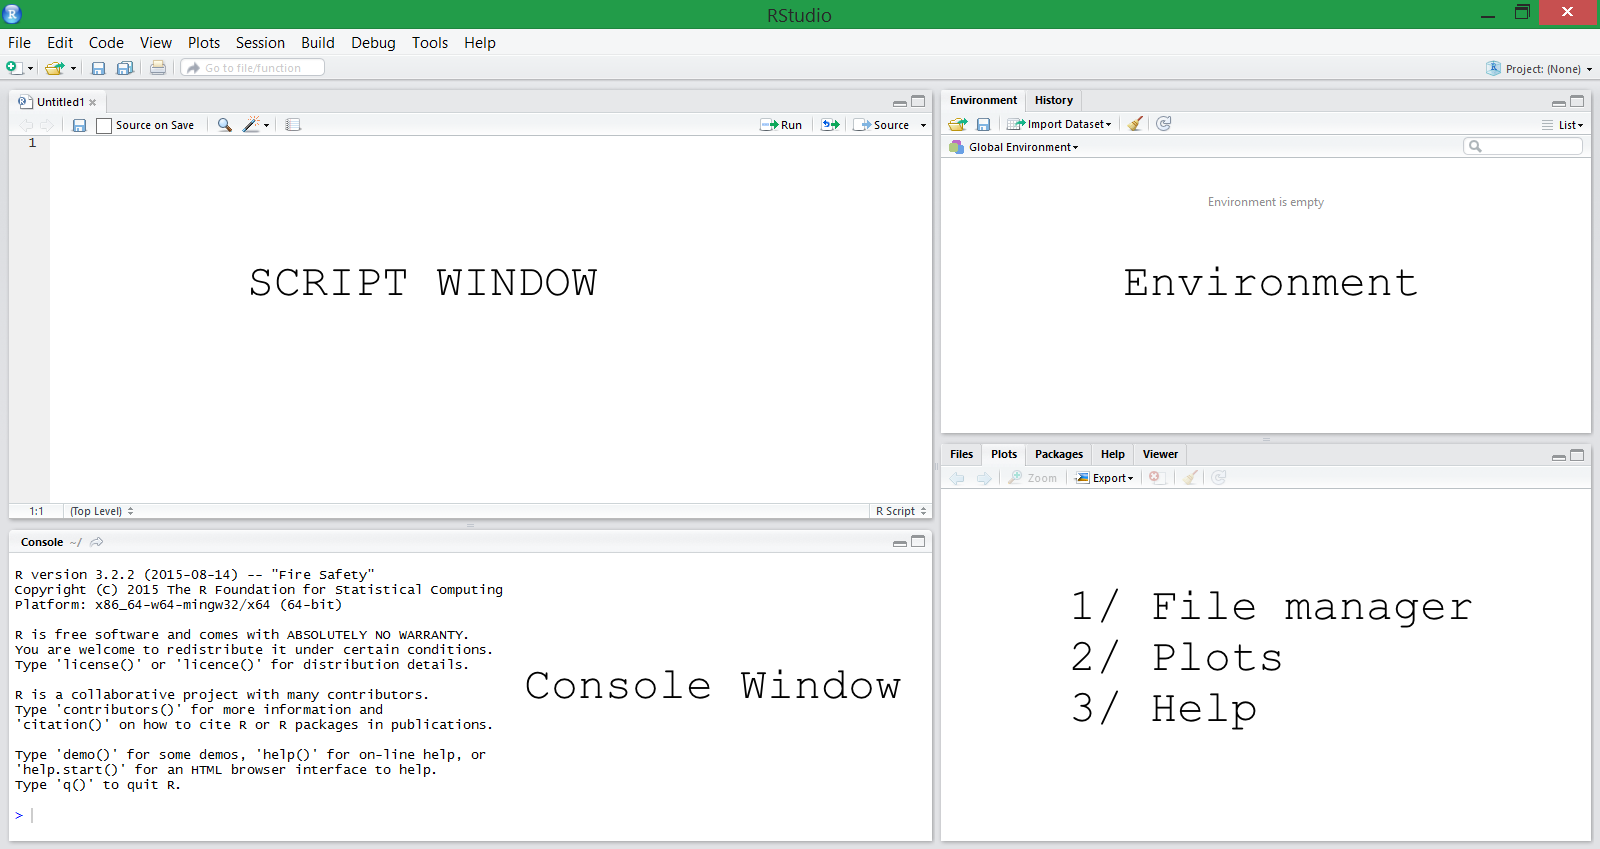
\includegraphics[width=\textwidth]{images/RStudioWindow}
\end{frame}
%%%%%%%%%%%%%%%%%%%%%%%%%%%%%%%%%%%%%%%%%%%%%%%%%%%%%%%%%%%%%%%%%%%%%%%%%%%%%%%%%%%%%%%%%%%%%%%%%%%%


%%%%%%%%%%%%%%%%%%%%%%%%%%%%%%%%%%%%%%%%%%%%%%%%%%%%%%%%%%%%%%%%%%%%%%%%%%%%%%%%%%%%%%%%%%%%%%%%%%%%
\begin{frame}[fragile]{RStudio IDE}
\begin{block}{Script Window}
Draft and save code.  Write a script to run in the console by CTRL+R or CTRL+Enter, or pressing Run.
\end{block}

\begin{block}{Console}
Where the code goes once run.  Shows {\color{blue} input (blue)}, output (black) and any {\color{red}errors or warnings (red)}. (different ``Themes" can be chosen to display different colours.
\end{block}

\begin{block}{Environment}
Shows saved variables and datasets
\end{block}

\begin{block}{File Browser/Plots/Help}
Show files in working directory and generated plots, help, open window.
\end{block}
\end{frame}
%%%%%%%%%%%%%%%%%%%%%%%%%%%%%%%%%%%%%%%%%%%%%%%%%%%%%%%%%%%%%%%%%%%%%%%%%%%%%%%%%%%%%%%%%%%%%%%%%%%%


%%%%%%%%%%%%%%%%%%%%%%%%%%%%%%%%%%%%%%%%%%%%%%%%%%%%%%%%%%%%%%%%%%%%%%%%%%%%%%%%%%%%%%%%%%%%%%%%%%%%
\begin{frame}[fragile]{Working Directory}
The \emph{working directory} is the ``home base'' of your R program.  All files are written to and read from the working directory.  There are two ways to do this:
\begin{enumerate}
\item Using the \emph{interface} by doing 
\begin{center}
\texttt{Session $\to$ Set Working Directory $\to$ Choose Directory}\\[1em]
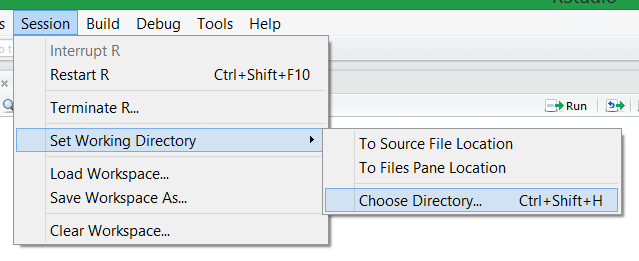
\includegraphics[width=.5\textwidth]{images/session}
\end{center}
\item Doing \texttt{setwd()} as in \texttt{\textquotedbl setwd(/Users/ivrbik)\textquotedbl}.  Note the working directory is retrieved with \texttt{getwd()}.
\end{enumerate}
\end{frame}
%%%%%%%%%%%%%%%%%%%%%%%%%%%%%%%%%%%%%%%%%%%%%%%%%%%%%%%%%%%%%%%%%%%%%%%%%%%%%%%%%%%%%%%%%%%%%%%%%%%%


%%%%%%%%%%%%%%%%%%%%%%%%%%%%%%%%%%%%%%%%%%%%%%%%%%%%%%%%%%%%%%%%%%%%%%%%%%%%%%%%%%%%%%%%%%%%%%%%%%%%
\begin{frame}[fragile]
The \texttt{print} function will \emph{print} to the console\\[2em]

\begin{Verbatim}[xleftmargin=2em, xrightmargin=1.5em, frame=single, numbers=left, label=print, framesep=0.5em]
> print("Hello world!")
[1] "Hello world!"
\end{Verbatim}
Print statements are often used in conjunction with {\tt paste()} functions\\[2em]

\begin{Verbatim}[xleftmargin=2em, xrightmargin=1.5em, frame=single, numbers=left, label=print and paste, framesep=0.5em]
> x <- 5
> print(paste("x =", x))
[1] "x = 5"
> print(paste("x", x, sep=" = "))
[1] "x = 5"
> print("x=",x) # doesn't work like python
[1] "x="
\end{Verbatim}
\end{frame}
%%%%%%%%%%%%%%%%%%%%%%%%%%%%%%%%%%%%%%%%%%%%%%%%%%%%%%%%%%%%%%%%%%%%%%%%%%%%%%%%%%%%%%%%%%%%%%%%%%%%


\begin{frame}[fragile]{Some notes}
\begin{itemize}
\item The \verb|>| character is  used to denote R \textit{input}.  \textit{Output} is given directly below (the number in the square brackets denotes corresponding element number in the object appearing beside it).
\begin{Verbatim}
> print(x) # where x holds the numbers 1 to 28
 [1]  1  2  3  4  5  6  7  8  9 10 11 12 13
[14] 14 15 16 17 18 
\end{Verbatim}
\item Like Python, R is case sensitive.\nl
\item Unlike Python, R in not that particular about white space and indent.
\begin{Verbatim}
>      x <- 5 # both OK!
> x <- 7
\end{Verbatim}
\end{itemize}

\end{frame}

%%%%%%%%%%%%%%%%%%%%%%%%%%%%%%%%%%%%%%%%%%%%%%%%%%%%%%%%%%%%%%%%%%%%%%%%%%%%%%%%%%%%%%%%%%%%%%%%%%%%
%\begin{frame}[fragile]
%\begin{question}
%Write a $R$ program that prints 
%\begin{enumerate}
%\item \texttt{\textquotedbl I am awesome!\textquotedbl}.
%\item \texttt{\textquotedbl I can program in R!\textquotedbl}.
%\item \texttt{\textquotedbl I can program in Python!\textquotedbl}.
%\item \texttt{\textquotedbl I can program in 2 languages! Can you?\textquotedbl}.
%\end{enumerate}
%\end{question}
%\end{frame}
%%%%%%%%%%%%%%%%%%%%%%%%%%%%%%%%%%%%%%%%%%%%%%%%%%%%%%%%%%%%%%%%%%%%%%%%%%%%%%%%%%%%%%%%%%%%%%%%%%%%


%%%%%%%%%%%%%%%%%%%%%%%%%%%%%%%%%%%%%%%%%%%%%%%%%%%%%%%%%%%%%%%%%%%%%%%%%%%%%%%%%%%%%%%%%%%%%%%%%%%%
\begin{frame}[fragile]{Basics of R}
\vfill
Lines can be be terminated by a semicolon (but they don't need to be) 
\begin{Verbatim}
> x <- 5; # both OK!
> x <- 5
\end{Verbatim}

\vfill
R commands may be separated either by a semi-colon or a newline.
\begin{Verbatim}[xleftmargin=0.3in]
> x <- 7
> y <- 3
> #or
> x <- 7; y<- 3
\end{Verbatim}
\vfill
Curly brackets $\{$ $\}$ are used to group commands together.
\begin{Verbatim}[xleftmargin=0.5in]
for (i in c(1,2,3)) {
  print(i)
  print(i + 1)
print(i - 1)  # indent doesn't matter
}
\end{Verbatim}
\vfill
\end{frame}
%%%%%%%%%%%%%%%%%%%%%%%%%%%%%%%%%%%%%%%%%%%%%%%%%%%%%%%%%%%%%%%%%%%%%%%%%%%%%%%%%%%%%%%%%%%%%%%%%%%%


%%%%%%%%%%%%%%%%%%%%%%%%%%%%%%%%%%%%%%%%%%%%%%%%%%%%%%%%%%%%%%%%%%%%%%%%%%%%%%%%%%%%%%%%%%%%%%%%%%%%
\begin{frame}[fragile]{Basics of R}
\vfill
\emph{Comment} lines begin with \#.  There is no multiline commenting in R.
\begin{Verbatim}[xleftmargin=2em, xrightmargin=1.5em]
> #This is a comment.
\end{Verbatim}
\vfill
\emph{Variables are assigned} with {\tt <- }  N.B. We can either use the {\tt =} or {\tt <-} for the assignment operator.  There is some debate on the \href{https://csgillespie.wordpress.com/2010/11/16/assignment-operators-in-r-vs/}{preferred syntax}

\begin{Verbatim}[xleftmargin=2em, xrightmargin=1.5em]
> x <- 4
> y <- 10
\end{Verbatim}
\vfill
To get \emph{help} do
\begin{Verbatim}[xleftmargin=2em, xrightmargin=1.5em]
> help(c)
> ?c
\end{Verbatim}
\vfill
\end{frame}
%%%%%%%%%%%%%%%%%%%%%%%%%%%%%%%%%%%%%%%%%%%%%%%%%%%%%%%%%%%%%%%%%%%%%%%%%%%%%%%%%%%%%%%%%%%%%%%%%%%%


%%%%%%%%%%%%%%%%%%%%%%%%%%%%%%%%%%%%%%%%%%%%%%%%%%%%%%%%%%%%%%%%%%%%%%%%%%%%%%%%%%%%%%%%%%%%%%%%%%%%
\begin{frame}[fragile]{Calculations in R}
R has the standard math operations +, -, *, /, and \textasciicircum{}.  Trigonometric functions \texttt{sin}, \texttt{cos}, and \texttt{tan}.  Exponential \texttt{exp}, \texttt{log} (base ten), \texttt{log10}.
\begin{multicols}{3}
\begin{Verbatim}[frame=single, xleftmargin=.5em, xrightmargin=.5em, commandchars=\\\{\}]
> 1+2
[1] 3
> 2*3
[1] 6
\end{Verbatim}
\newpage
\begin{Verbatim}[frame=single, xleftmargin=.5em, xrightmargin=.5em, commandchars=\\\{\}]
> 6/2
[1] 3
> 2^3
8
\end{Verbatim}
\newpage
\begin{Verbatim}[frame=single, xleftmargin=.5em, xrightmargin=0em, commandchars=\\\{\}]
> sin(pi)
[1] 1.224647e-16
> log10(100)
[1] 2
\end{Verbatim}
\end{multicols}
Note \texttt{pi} has a value but is \emph{not a protected name}.  Further note \texttt{pi}'s value is \emph{approximate}.
\end{frame}
%%%%%%%%%%%%%%%%%%%%%%%%%%%%%%%%%%%%%%%%%%%%%%%%%%%%%%%%%%%%%%%%%%%%%%%%%%%%%%%%%%%%%%%%%%%%%%%%%%%%


\begin{frame}[fragile]{Basic Operations for Vectors}
We can also perform basic operations on vectors:
\begin{center}
\begin{tabular}{ll}
Operation & Command \\\hline 
natural log & \verb!log(x)!\\
Exponent & \verb!exp(x)!\\
Log base 10 & \verb!log10(x)!\\
Absolute value & \verb!abs(x)!\\
Square root & \verb!sqrt(x)!\\
Sum & \verb!sum(x)!\\
Number of elements in $x$  & \verb!length(x)!\\
\end{tabular}
\end{center}
\end{frame}


\begin{frame}[fragile]{}
\begin{center}
\begin{tabular}{ll}
Unique elements of $x$ & \verb!unique(x)!\\
Mean & \verb!mean(x)!\\
Variance & \verb!var(x)!\\
Standard Deviation & \verb!sd(x)!\\
Minimum value & \verb!min(x)!\\
Maximum value & \verb!max(x)!\\
Smallest and largest values  & \verb!range(x)!\\
median & \verb!median(x)!\\
Basic statistical summary & \verb!summary(x)!\\
Sort & \verb!sort(x)!\\
\end{tabular}
\end{center}
\end{frame}



%%%%%%%%%%%%%%%%%%%%%%%%%%%%%%%%%%%%%%%%%%%%%%%%%%%%%%%%%%%%%%%%%%%%%%%%%%%%%%%%%%%%%%%%%%%%%%%%%%%%
\begin{frame}[fragile]
\begin{question}
How many of the following are true?
\begin{enumerate}
\item R is case-sensitive.
\item A command in R can be terminated by a semi-colon. 
\item Indentation is the syntax used to group statements together. 
\item A single line comment starts with \#. 
\end{enumerate}
\begin{multicols}{5}
\begin{enumerate}[A)]
\item 0
\item 1
\item 2
\item 3
\item 4
\end{enumerate}
\end{multicols}
\end{question}
\end{frame}


\begin{frame}<handout:0>[fragile]
\begin{question}
How many of the following are true?
\begin{enumerate}
\item R is case-sensitive. \onslide<+->\pcmark
\item A command in R can be terminated by a semi-colon. \pcmark
\item Indentation is the syntax used to group statements together. \pxmark
\item A single line comment starts with \#. \pcmark
\end{enumerate}
\begin{multicols}{5}
\begin{enumerate}[A)]
\item 0
\item 1
\item 2
\item \tans{6}{3}
\item 4
\end{enumerate}
\end{multicols}
\end{question}
\end{frame}


%%%%%%%%%%%%%%%%%%%%%%%%%%%%%%%%%%%%%%%%%%%%%%%%%%%%%%%%%%%%%%%%%%%%%%%%%%%%%%%%%%%%%%%%%%%%%%%%%%%%


%%%%%%%%%%%%%%%%%%%%%%%%%%%%%%%%%%%%%%%%%%%%%%%%%%%%%%%%%%%%%%%%%%%%%%%%%%%%%%%%%%%%%%%%%%%%%%%%%%%%

\begin{frame}{R Data Types}
\begin{description}
\item[Numeric] Decimal values
\item[Integer] Can be created using as.integer()
\item[Complex] Complex values  (i.e. a+bi)
\item[Logical] TRUE/FALSE. Can be denoted using T/F (Boolean variables)
\item[Character] String values denoted with single or double quotes.  

\end{description}


\end{frame}



\begin{frame}[fragile]{R Data Types}
\begin{Verbatim}[xleftmargin=2em, xrightmargin=1.5em, frame=single, numbers=left, label=Typing checking in R, framesep=0.5em]
> class(1)
[1] "numeric"
> class(as.integer(1))
[1] "integer"
> z = 1 + 2i; class(z)
[1] "complex"
> class(TRUE) # notice all in caps! 
[1] "logical"
> class("irene")
[1] "character"
\end{Verbatim}
We could also use {\tt typeof()}, see the \href{https://stat.ethz.ch/R-manual/R-devel/doc/manual/R-lang.html#Objects}{R Language Definition} manual, and more about their differences \href{http://rfunction.com/archives/770}{here}
\end{frame}

%%%%%%%%%%%%%%%%%%%%%%%%%%%%%%%%%%%%%%%%%%%%%%%%%%%%%%%%%%%%%%%%%%%%%%%%%%%%%%%%%%%%%%%%%%%%%%%%%%%%


%%%%%%%%%%%%%%%%%%%%%%%%%%%%%%%%%%%%%%%%%%%%%%%%%%%%%%%%%%%%%%%%%%%%%%%%%%%%%%%%%%%%%%%%%%%%%%%%%%%%
\begin{frame}[fragile]{Try it: in R}
\begin{question}
In an R program
\begin{enumerate}
\item Make a comment with your name and student number.
\item Calculate the following $4 \times 5 - 12^3$, ${\rm e}^{3 \times 4}$, $\sin(4\pi-6)$.
\item Guess then check with \texttt{class} the types of the following variables
\begin{Verbatim}[xleftmargin=2em, xrightmargin=1.5em, framesep=0.5em]
> var1 <- FALSE
> var2 <- T
> var2b <- "TRUE"
> var3 <- 3^4 - 10
> var4 <- "Hello World"
\end{Verbatim}
\end{enumerate}
\end{question}
\end{frame}
%%%%%%%%%%%%%%%%%%%%%%%%%%%%%%%%%%%%%%%%%%%%%%%%%%%%%%%%%%%%%%%%%%%%%%%%%%%%%%%%%%%%%%%%%%%%%%%%%%%%



\begin{frame}[fragile]{Data structures}
\begin{itemize}
\item R has a wide variety of data structures including:
\begin{itemize}
\item scalars
\item vectors (numerical, character, logical)
\item matrices
\item data frames, and
\item lists.
\end{itemize}
\end{itemize}
\end{frame}



\begin{frame}[fragile]{Vectors}
\begin{itemize}
\item A vector is the most basic data structure in \R and can be of two types:
\begin{itemize}
\item atomic vectors (containing all the same type of data)
\item lists (can contain a mixture of different types of data)
\end{itemize}
\item As we did in the examples above, you can create a vector using \texttt{c} (see {\tt ?c} for more details on this \textit{combine} function)
\end{itemize}
\end{frame}


\begin{frame}[fragile]{Vectors}
Atomic Vectors can be vectors characters, logical, integers or numeric.
\begin{Verbatim}[xleftmargin=0.3in]
# example of a numeric vector:
y=c(2,3,0,3,1,0,0,1)
# example of a character vector:
letters<-c('A','B','C')
# example of a logical vector:
lvec <- c(TRUE, FALSE, FALSE)
\end{Verbatim}

\end{frame}


\begin{frame}[fragile]{Vectors}
Numeric vectors can be created a number of different ways. 
\begin{Verbatim}[xleftmargin=0.3in]
# Ceate a vector of size 10, where each element is a 2:
y=rep(2,10)
# This specifies a sequence of integers:
y=3:12
#This specifies a sequence of real numbers:
z=seq(from=1,to=2,by=0.1)
#This specifies a sequence of real numbers:
z=seq(from=2,to=1,by=-0.1)
\end{Verbatim}
\begin{alertblock}{The end number (specified by the {\tt to} argument) \textit{is} inclusive!}
%Notice that the end number \textit{is} included in the sequence of numbers generated by \R
\end{alertblock}

\end{frame}


\begin{frame}[fragile]{Indexing Vectors}
To index an element from a vector, use single square brackets
\begin{Verbatim}[xleftmargin=0.3in]
> z = c("apples","bananas","oranges", "pineapples")
> z[1]
[1] "apples"
> z[2:3]
[1] "bananas" "oranges"
> z[c(4,2)] # for selecting non-contiguous elements
[1] "pineapples" "bananas"   
> z[-1] # removes the first item
[1] "bananas"    "oranges"    "pineapples"
\end{Verbatim}
\begin{alertblock}{Notice that the index begins at 1}
Also notice the difference in the \verb|[-1]| notation.
\end{alertblock}

\end{frame}


\begin{frame}[fragile]{}
We have the option of including names for our vector elements (similar to a Python dictionary)
\begin{Verbatim}[xleftmargin=0.3in]
z = c(123456, 25, 2019)
names(z) <- c("studentID","age","year")
z["studentID"] # same as z[1]
z[c("age, year")] # wont work like z[c(2,3)]
z[c(FALSE, TRUE, TRUE)] # will work 
z[-"year"] # wont work like z[-3]
\end{Verbatim}
\end{frame}


\begin{frame}[fragile]{}
To add a new element/delete/replace an element:
\begin{Verbatim}[xleftmargin=0.4in]
> z = c("first","second","third", "fourth")
> # adds a fith element and replaces the second
> z[5] = "fifth" # doesn't need to exist before we assign
> z[2] = "2nd"
> z
[1] "first"  "2nd"    "third"  "fourth" "fifth" 
> #removes the second element
> (z = z[-2])
[1] "first"  "third"  "fourth" "fifth" 
\end{Verbatim}


\end{frame}


\begin{frame}[fragile]{}
Notice what happens if we add a 10th element to z (without specifying elements 6--9):
\begin{Verbatim}[xleftmargin=0.4in]
> z[10] = "tenth"
> z
 [1] "first"  "third"  "fourth" "fifth"  NA      
 [6] NA       NA       NA       NA       "tenth" 
 \end{Verbatim}
We can also add new named elements
\begin{Verbatim}[xleftmargin=0.4in]
> z = c(123456, 25, 2019)
> names(z) <- c("studentID","age","year")
> # adds a forth element with the students major
> z["major"] = "COSC"
> z
studentID       age      year     major 
 "123456"      "25"    "2019"    "COSC" 
 \end{Verbatim}
\end{frame}


\begin{frame}[fragile]{Vector operations}
Notice that operations performed on vectors get computed on each element of the vector (similar to {\tt map} iin Python)
\begin{Verbatim}[xleftmargin=0.4in]
> x <- 1:10
> y <- 11:20
> x*2
 [1]  2  4  6  8 10 12 14 16 18 20
> x+y
 [1] 12 14 16 18 20 22 24 26 28 30
\end{Verbatim}
\end{frame}


\begin{frame}[fragile]{Matrices}
\begin{itemize}
\item While we can view matrices as column vectors stacked side by side or row vectors stack one on top of another, matrices are really just a vector in \R.
\item The main difference between matrices and the vectors discussed in the previous slides is that a matrix has a \define{dimension} (like {\tt numpy arrays} in Python)
\item The dimenions can be found using the {\tt dim()} function. 
\end{itemize}
\end{frame}


\begin{frame}[fragile]{Matrices}
\begin{Verbatim}[xleftmargin=0.4in]
> (m <- matrix(1:8, nrow = 2, ncol = 4))
     [,1] [,2] [,3] [,4]
[1,]    1    3    5    7
[2,]    2    4    6    8
> dim(m) # gives the number or rows and columns
[1] 2 4
> class(m)
[1] "matrix"
\end{Verbatim}
\end{frame}

\begin{frame}[fragile]{Matrices}
\begin{itemize}
\item By default, matrices are constructed columnwise.  
\item You can always change to row-wise by specifying {\tt byrow=TRUE}
\end{itemize}
\begin{knitrout}\footnotesize
\definecolor{shadecolor}{rgb}{0.969, 0.969, 0.969}\color{fgcolor}\begin{kframe}
\begin{alltt}
\hlstd{(m} \hlkwb{<-} \hlkwd{matrix}\hlstd{(}\hlnum{1}\hlopt{:}\hlnum{6}\hlstd{,} \hlkwc{nrow}\hlstd{=}\hlnum{2}\hlstd{,} \hlkwc{ncol} \hlstd{=}\hlnum{3}\hlstd{))} \hlcom{# fill columnwise}
\end{alltt}
\begin{verbatim}
##      [,1] [,2] [,3]
## [1,]    1    3    5
## [2,]    2    4    6
\end{verbatim}
\begin{alltt}
\hlstd{(m} \hlkwb{<-} \hlkwd{matrix}\hlstd{(}\hlnum{1}\hlopt{:}\hlnum{6}\hlstd{,} \hlkwc{nrow}\hlstd{=}\hlnum{2}\hlstd{,} \hlkwc{ncol} \hlstd{=}\hlnum{3}\hlstd{,} \hlkwc{byrow}\hlstd{=}\hlnum{TRUE}\hlstd{))} \hlcom{#fill row-wise}
\end{alltt}
\begin{verbatim}
##      [,1] [,2] [,3]
## [1,]    1    2    3
## [2,]    4    5    6
\end{verbatim}
\end{kframe}
\end{knitrout}
\end{frame}


\begin{frame}[fragile]{Named Matrices}
We may also choose to name our rows and columns
\begin{knitrout}\footnotesize
\definecolor{shadecolor}{rgb}{0.969, 0.969, 0.969}\color{fgcolor}\begin{kframe}
\begin{alltt}
\hlkwd{rownames}\hlstd{(m)} \hlkwb{=} \hlkwd{c}\hlstd{(}\hlstr{"row1"}\hlstd{,} \hlstr{"row2"}\hlstd{)}
\hlkwd{colnames}\hlstd{(m)} \hlkwb{=} \hlkwd{c}\hlstd{(}\hlstr{"col1"}\hlstd{,} \hlstr{"col2"}\hlstd{,} \hlstr{"col3"}\hlstd{)}
\hlstd{m}
\end{alltt}
\begin{verbatim}
##      col1 col2 col3
## row1    1    2    3
## row2    4    5    6
\end{verbatim}
\end{kframe}
\end{knitrout}
\end{frame}


\begin{frame}[fragile]{Indexing}
\begin{itemize}
\item To index an element from a matrix, we can again use square brackets, but we need to specify TWO numbers {\tt[row, col]}.
\item  If we want to extract an entire row, we'll leave the {\tt col} field blank (indicating we want all colums).
\item  If we want to extract an entire column, we'll leave the {\tt row} field blank (indicating we want all rows).
\end{itemize}
\end{frame}

\begin{frame}[fragile]{Indexing}
The following extracts a column, row, and cell from matrix {\tt m},
\begin{knitrout}\footnotesize
\definecolor{shadecolor}{rgb}{0.969, 0.969, 0.969}\color{fgcolor}\begin{kframe}
\begin{alltt}
\hlcom{# extract the third column of m}
\hlstd{m[,}\hlnum{3}\hlstd{]}
\end{alltt}
\begin{verbatim}
## row1 row2 
##    3    6
\end{verbatim}
\begin{alltt}
\hlcom{# extract the first row of m}
\hlstd{m[}\hlnum{1}\hlstd{,]}
\end{alltt}
\begin{verbatim}
## col1 col2 col3 
##    1    2    3
\end{verbatim}
\begin{alltt}
\hlcom{# extract the element in the 1st row and 3rd column}
\hlstd{m[}\hlnum{1}\hlstd{,}\hlnum{3}\hlstd{]}
\end{alltt}
\begin{verbatim}
## [1] 3
\end{verbatim}
\end{kframe}
\end{knitrout}
\end{frame}

\begin{frame}[fragile]{}
Alternatively we could call them by name
\begin{knitrout}\footnotesize
\definecolor{shadecolor}{rgb}{0.969, 0.969, 0.969}\color{fgcolor}\begin{kframe}
\begin{alltt}
\hlcom{# extract the third column of m}
\hlstd{m[,}\hlstr{"col3"}\hlstd{]} \hlcom{# same as m[,3]}
\end{alltt}
\begin{verbatim}
## row1 row2 
##    3    6
\end{verbatim}
\begin{alltt}
\hlcom{# extract the first row of m}
\hlstd{m[}\hlstr{"row1"}\hlstd{,]} \hlcom{# same as m[1,]}
\end{alltt}
\begin{verbatim}
## col1 col2 col3 
##    1    2    3
\end{verbatim}
\begin{alltt}
\hlcom{# extract the element in the 1st row and 3rd column}
\hlstd{m[}\hlstr{"row1"}\hlstd{,}\hlstr{"col3"}\hlstd{]} \hlcom{# same as m[1,3]}
\end{alltt}
\begin{verbatim}
## [1] 3
\end{verbatim}
\end{kframe}
\end{knitrout}
\end{frame}


\begin{frame}[fragile]{Indexing}
Note that we can also use one number (tricker this way)
\begin{knitrout}\footnotesize
\definecolor{shadecolor}{rgb}{0.969, 0.969, 0.969}\color{fgcolor}\begin{kframe}
\begin{alltt}
\hlstd{(m} \hlkwb{=} \hlkwd{matrix}\hlstd{(}\hlnum{11}\hlopt{:}\hlnum{4}\hlstd{,} \hlnum{2}\hlstd{,}\hlnum{4}\hlstd{))}
\end{alltt}
\begin{verbatim}
##      [,1] [,2] [,3] [,4]
## [1,]   11    9    7    5
## [2,]   10    8    6    4
\end{verbatim}
\begin{alltt}
\hlstd{m[}\hlnum{8}\hlstd{]} \hlcom{# extracts the 8th element in m}
\end{alltt}
\begin{verbatim}
## [1] 4
\end{verbatim}
\begin{alltt}
\hlstd{(mVector} \hlkwb{=} \hlkwd{as.numeric}\hlstd{(m))}
\end{alltt}
\begin{verbatim}
## [1] 11 10  9  8  7  6  5  4
\end{verbatim}
\begin{alltt}
\hlstd{mVector[}\hlnum{8}\hlstd{]}
\end{alltt}
\begin{verbatim}
## [1] 4
\end{verbatim}
\end{kframe}
\end{knitrout}
\end{frame}

\begin{frame}[fragile]{Indexing}
Like the vectors discussed earlier, matices fall under the atomic vector category and therefore can only store data of one type:
\begin{knitrout}\footnotesize
\definecolor{shadecolor}{rgb}{0.969, 0.969, 0.969}\color{fgcolor}\begin{kframe}
\begin{alltt}
\hlstd{m} \hlkwb{=} \hlkwd{matrix}\hlstd{(}\hlkwd{c}\hlstd{(}\hlstr{"bananas"}\hlstd{,} \hlnum{2}\hlstd{,} \hlnum{TRUE}\hlstd{,} \hlnum{0}\hlstd{),}  \hlkwc{nrow}\hlstd{=}\hlnum{2}\hlstd{,} \hlkwc{ncol}\hlstd{=}\hlnum{2}\hlstd{)}
\hlcom{# notice how all coerce to characters:}
\hlstd{m}
\end{alltt}
\begin{verbatim}
##      [,1]      [,2]  
## [1,] "bananas" "TRUE"
## [2,] "2"       "0"
\end{verbatim}
\end{kframe}
\end{knitrout}
\end{frame}




\begin{frame}[fragile]{lists}
\begin{itemize}
\item
If we want our vector to contain objects of different data types we need to create a list.
\item We can think of lists as a special type of vector that can mix data types and  structures
\end{itemize}
\end{frame}

\begin{frame}[fragile]{}

\begin{knitrout}\scriptsize
\definecolor{shadecolor}{rgb}{0.969, 0.969, 0.969}\color{fgcolor}\begin{kframe}
\begin{alltt}
\hlstd{(x} \hlkwb{=} \hlkwd{list}\hlstd{(}\hlstr{"apple"}\hlstd{,} \hlstr{"banana"}\hlstd{,} \hlnum{2}\hlstd{,} \hlnum{TRUE}\hlstd{,} \hlnum{4}\hlstd{,} \hlstr{"four"}\hlstd{))}
\end{alltt}
\begin{verbatim}
## [[1]]
## [1] "apple"
## 
## [[2]]
## [1] "banana"
## 
## [[3]]
## [1] 2
## 
## [[4]]
## [1] TRUE
## 
## [[5]]
## [1] 4
## 
## [[6]]
## [1] "four"
\end{verbatim}
\end{kframe}
\end{knitrout}
\end{frame}


\begin{frame}[fragile]{lists}
Unlike vectors, the member of a list are accessed using double square brackets:
\begin{knitrout}\footnotesize
\definecolor{shadecolor}{rgb}{0.969, 0.969, 0.969}\color{fgcolor}\begin{kframe}
\begin{alltt}
\hlstd{x[[}\hlnum{1}\hlstd{]]} \hlcom{# first member}
\end{alltt}
\begin{verbatim}
## [1] "apple"
\end{verbatim}
\begin{alltt}
\hlstd{x[[}\hlnum{2}\hlstd{]]} \hlcom{# second member, and so on ...}
\end{alltt}
\begin{verbatim}
## [1] "banana"
\end{verbatim}
\end{kframe}
\end{knitrout}
\end{frame}

\begin{frame}[fragile]{lists}
\begin{itemize}
\item While I have specified each member to be a single word/number/logical, we could also have specified them to be vectors or matrices. 
\item To index the elements within the members of a list we use single square brackets (usually nested after double square brackets)
\end{itemize}
\end{frame}


\begin{frame}[fragile]{lists}
\begin{knitrout}\footnotesize
\definecolor{shadecolor}{rgb}{0.969, 0.969, 0.969}\color{fgcolor}\begin{kframe}
\begin{alltt}
\hlstd{y} \hlkwb{=} \hlkwd{list}\hlstd{(}\hlkwd{c}\hlstd{(}\hlstr{"apples"}\hlstd{,} \hlstr{"banana"}\hlstd{,} \hlstr{"four"}\hlstd{),} \hlkwd{c}\hlstd{(}\hlnum{2}\hlstd{,}\hlnum{4}\hlstd{),} \hlnum{TRUE}\hlstd{)}
\hlstd{y}
\end{alltt}
\begin{verbatim}
## [[1]]
## [1] "apples" "banana" "four"  
## 
## [[2]]
## [1] 2 4
## 
## [[3]]
## [1] TRUE
\end{verbatim}
\end{kframe}
\end{knitrout}
\end{frame}

\begin{frame}[fragile]{lists}
\begin{knitrout}\footnotesize
\definecolor{shadecolor}{rgb}{0.969, 0.969, 0.969}\color{fgcolor}\begin{kframe}
\begin{alltt}
\hlstd{y[[}\hlnum{1}\hlstd{]][}\hlnum{3}\hlstd{]} \hlcom{# the third element of the first member of y}
\end{alltt}
\begin{verbatim}
## [1] "four"
\end{verbatim}
\begin{alltt}
\hlstd{y[[}\hlnum{2}\hlstd{]][}\hlnum{1}\hlstd{]} \hlcom{# the first element of the second member of y}
\end{alltt}
\begin{verbatim}
## [1] 2
\end{verbatim}
\begin{alltt}
\hlstd{y[[}\hlnum{1}\hlstd{]][}\hlnum{4}\hlstd{]} \hlcom{# calling something that does not exist }
\end{alltt}
\begin{verbatim}
## [1] NA
\end{verbatim}
\end{kframe}
\end{knitrout}
\end{frame}

\begin{frame}[fragile]{Named lists}
Alternatively we could have names for our list members
\begin{knitrout}\footnotesize
\definecolor{shadecolor}{rgb}{0.969, 0.969, 0.969}\color{fgcolor}\begin{kframe}
\begin{alltt}
\hlstd{numbers}\hlkwb{=} \hlkwd{c}\hlstd{(}\hlnum{2}\hlstd{,}\hlnum{4}\hlstd{)} \hlcom{# can define the member outside first}
\hlstd{y} \hlkwb{=} \hlkwd{list}\hlstd{(}\hlkwc{words}\hlstd{=}\hlkwd{c}\hlstd{(}\hlstr{"apples"}\hlstd{,} \hlstr{"banana"}\hlstd{,} \hlstr{"four"}\hlstd{),}
         \hlstd{numbers,} \hlkwc{logicals}\hlstd{=}\hlnum{TRUE}\hlstd{)}
\hlstd{y}\hlopt{$}\hlstd{words} \hlcom{# same this as y[[1]]}
\end{alltt}
\begin{verbatim}
## [1] "apples" "banana" "four"
\end{verbatim}
\begin{alltt}
\hlstd{y}\hlopt{$}\hlstd{numbers} \hlcom{# same this as y[[2]]}
\end{alltt}
\begin{verbatim}
## NULL
\end{verbatim}
\begin{alltt}
\hlstd{y}\hlopt{$}\hlstd{logicals} \hlcom{# same this as y[[3]]}
\end{alltt}
\begin{verbatim}
## [1] TRUE
\end{verbatim}
\end{kframe}
\end{knitrout}
\end{frame}


\begin{frame}[fragile]{}
We could also name the list members after they have been assigned
\begin{knitrout}\footnotesize
\definecolor{shadecolor}{rgb}{0.969, 0.969, 0.969}\color{fgcolor}\begin{kframe}
\begin{alltt}
\hlstd{y} \hlkwb{=} \hlkwd{list}\hlstd{(}\hlkwd{c}\hlstd{(}\hlstr{"apples"}\hlstd{,} \hlstr{"banana"}\hlstd{,} \hlstr{"four"}\hlstd{),}
         \hlkwd{c}\hlstd{(}\hlnum{2}\hlstd{,}\hlnum{4}\hlstd{),} \hlnum{TRUE}\hlstd{)}
\hlkwd{names}\hlstd{(y)} \hlkwb{<-} \hlkwd{c}\hlstd{(}\hlstr{"words"}\hlstd{,}\hlstr{"numbers"}\hlstd{,}\hlstr{"logicals"}\hlstd{)}
\hlstd{y}
\end{alltt}
\begin{verbatim}
## $words
## [1] "apples" "banana" "four"  
## 
## $numbers
## [1] 2 4
## 
## $logicals
## [1] TRUE
\end{verbatim}
\end{kframe}
\end{knitrout}
\end{frame}

\begin{frame}[fragile]{lists}
We can index members of lists using the integer index numbers OR their member names (in quotations) 
\begin{knitrout}\footnotesize
\definecolor{shadecolor}{rgb}{0.969, 0.969, 0.969}\color{fgcolor}\begin{kframe}
\begin{alltt}
\hlstd{y}\hlopt{$}\hlstd{words}
\end{alltt}
\begin{verbatim}
## [1] "apples" "banana" "four"
\end{verbatim}
\begin{alltt}
\hlstd{y[[}\hlstr{"words"}\hlstd{]]}
\end{alltt}
\begin{verbatim}
## [1] "apples" "banana" "four"
\end{verbatim}
\begin{alltt}
\hlstd{y[[}\hlnum{4}\hlstd{]]}
\end{alltt}


{\ttfamily\noindent\bfseries\color{errorcolor}{\#\# Error in y[[4]]: subscript out of bounds}}\begin{alltt}
\hlcom{# the following are not valid:}
\hlcom{# y$4 }
\hlcom{# y[[words]]}
\end{alltt}
\end{kframe}
\end{knitrout}
\end{frame}





\begin{frame}[fragile]{lists}
We can modify its content/add new content directly either using {\tt [[]]} with numbers or {\tt \$} with member names. 
\begin{knitrout}\footnotesize
\definecolor{shadecolor}{rgb}{0.969, 0.969, 0.969}\color{fgcolor}\begin{kframe}
\begin{alltt}
\hlstd{y}\hlopt{$}\hlstd{words[}\hlnum{3}\hlstd{]} \hlkwb{=} \hlstr{"oranges"}\hlcom{#replace the 3rd element of the 1st member}
\hlstd{y[[}\hlnum{1}\hlstd{]][}\hlnum{4}\hlstd{]} \hlkwb{=} \hlstr{"pineapples"}\hlcom{#add a 4th element to the 1st member}
\hlstd{y[[}\hlnum{4}\hlstd{]]} \hlkwb{=} \hlkwd{c}\hlstd{(}\hlnum{0}\hlstd{,}\hlnum{1}\hlstd{,}\hlnum{1}\hlstd{,}\hlnum{0}\hlstd{)} \hlcom{# add a forth member to y}
\hlstd{y}\hlopt{$}\hlstr{"fifth"} \hlkwb{=} \hlnum{3}\hlopt{:}\hlnum{12} \hlcom{# add a fifth member to y (named "fifth")}
\end{alltt}
\end{kframe}
\end{knitrout}
\end{frame}



\begin{frame}[fragile]{Data Frames}
\begin{itemize}
\item Data frames are perhaps the most used data structure used in statistics. 
\item Like list, they can store different data types.
\item Futhermore, they can contain  additional attributes such as column and row names. \item When combining vectors in a data frame  all must have the same size (i.e. length).  \item Missing observations will be recorded as \texttt{NA}.
\end{itemize}
\end{frame}

\begin{frame}[fragile]{Data Frames}
Here is an example of how to create a data frame and add to it: 
\begin{knitrout}\footnotesize
\definecolor{shadecolor}{rgb}{0.969, 0.969, 0.969}\color{fgcolor}\begin{kframe}
\begin{alltt}
\hlstd{Person}\hlkwb{=}\hlkwd{c}\hlstd{(}\hlstr{'John'}\hlstd{,} \hlstr{'Jill'}\hlstd{,} \hlstr{'Jack'}\hlstd{)}
\hlstd{Grade}\hlkwb{=}\hlkwd{c}\hlstd{(}\hlstr{'45'}\hlstd{,}\hlstr{'92'}\hlstd{,}\hlstr{'91'}\hlstd{)}
\hlstd{(Lab}\hlkwb{=}\hlkwd{data.frame}\hlstd{(Person, Grade))}
\end{alltt}
\begin{verbatim}
##   Person Grade
## 1   John    45
## 2   Jill    92
## 3   Jack    91
\end{verbatim}
\end{kframe}
\end{knitrout}
\end{frame}

\begin{frame}[fragile]{Data Frames}
Like matrices, we can create column and row names
\begin{knitrout}\footnotesize
\definecolor{shadecolor}{rgb}{0.969, 0.969, 0.969}\color{fgcolor}\begin{kframe}
\begin{alltt}
\hlkwd{colnames}\hlstd{(Lab)} \hlcom{# adopted from the variable names inputed}
\end{alltt}
\begin{verbatim}
## [1] "Person" "Grade"
\end{verbatim}
\begin{alltt}
\hlkwd{rownames}\hlstd{(Lab)} \hlcom{# default to increasing integers}
\end{alltt}
\begin{verbatim}
## [1] "1" "2" "3"
\end{verbatim}
\begin{alltt}
\hlcom{# we could also add row names if we choose}
\hlkwd{rownames}\hlstd{(Lab)} \hlkwb{=} \hlkwd{c}\hlstd{(}\hlstr{"Student1"}\hlstd{,} \hlstr{"Student2"}\hlstd{,} \hlstr{"Student3"}\hlstd{)}
\hlstd{Lab}
\end{alltt}
\begin{verbatim}
##          Person Grade
## Student1   John    45
## Student2   Jill    92
## Student3   Jack    91
\end{verbatim}
\end{kframe}
\end{knitrout}
\end{frame}

\begin{frame}[fragile]{Data Frames}
Unlike matrices, we can extract a column of this data.frame we use the {\tt \$} notation:
\begin{knitrout}\footnotesize
\definecolor{shadecolor}{rgb}{0.969, 0.969, 0.969}\color{fgcolor}\begin{kframe}
\begin{alltt}
\hlstd{Lab}\hlopt{$}\hlstd{Person}
\end{alltt}
\begin{verbatim}
## [1] John Jill Jack
## Levels: Jack Jill John
\end{verbatim}
\begin{alltt}
\hlstd{Lab}\hlopt{$}\hlstd{Grade}
\end{alltt}
\begin{verbatim}
## [1] 45 92 91
## Levels: 45 91 92
\end{verbatim}
\begin{alltt}
\hlcom{# N.B. This does not work for rows:}
\hlstd{Lab}\hlopt{$}\hlstd{Student1}
\end{alltt}
\begin{verbatim}
## NULL
\end{verbatim}
\end{kframe}
\end{knitrout}
\end{frame}

\begin{frame}[fragile]{Aside}{Smart Autofill}
\begin{itemize}
\item In some situations, \R will try to autocomplete commands for us.  When you begin to type {\tt Lab\$} for instance, you will see the options for the column names appear.
\item You can use the arrow keys on your keyboard to navigate through the options.
\item Press \keystroke{ENTER} when you land on the option you want.
\end{itemize}
\end{frame}

\begin{frame}[fragile]{Data Frames}
Adding a column to the data frame is as easy as typing:
\begin{knitrout}\footnotesize
\definecolor{shadecolor}{rgb}{0.969, 0.969, 0.969}\color{fgcolor}\begin{kframe}
\begin{alltt}
\hlstd{Lab}\hlopt{$}\hlstd{Passed}\hlkwb{=}\hlkwd{c}\hlstd{(}\hlnum{FALSE}\hlstd{,}\hlnum{TRUE}\hlstd{,}\hlnum{TRUE}\hlstd{)}
\hlstd{Lab}
\end{alltt}
\begin{verbatim}
##          Person Grade Passed
## Student1   John    45  FALSE
## Student2   Jill    92   TRUE
## Student3   Jack    91   TRUE
\end{verbatim}
\end{kframe}
\end{knitrout}
\end{frame}

\begin{frame}[fragile]{Attributes}
\begin{itemize}
\item Each of these objects have so-called \emph{attributes}. %Think of attributes as their ‘identifier’, a name or number which aptly identifies them. 
\item Here are some examples of attributes:
\begin{enumerate}
\item names, dimension names
\item dimensions
\item class
\item length
\end{enumerate}
\end{itemize}
\end{frame}


\begin{frame}[fragile]{Attributes}
\begin{knitrout}\footnotesize
\definecolor{shadecolor}{rgb}{0.969, 0.969, 0.969}\color{fgcolor}\begin{kframe}
\begin{alltt}
\hlkwd{attributes}\hlstd{(Lab)} \hlcom{# data vector defined in previous example}
\end{alltt}
\begin{verbatim}
## $names
## [1] "Person" "Grade"  "Passed"
## 
## $row.names
## [1] "Student1" "Student2" "Student3"
## 
## $class
## [1] "data.frame"
\end{verbatim}
\begin{alltt}
\hlkwd{attributes}\hlstd{(m)} \hlcom{# matrix defined previously}
\end{alltt}
\begin{verbatim}
## $dim
## [1] 2 2
\end{verbatim}
\end{kframe}
\end{knitrout}
\end{frame}



\begin{frame}{Data Entry}
\begin{itemize}
\item Data entry can be either done by hand (impractical), or loaded from an existing file. 
\item  {\tt read.table} is a convenient way of reading data into \R and storing it to a data frame.
\item The data should be formated such that each rows contains information regarding one subject with data separated by white space/commas/tabs/.
\item The first line may (or may not) contain a {\tt header} with the names of the variables in each column.
\end{itemize}
\end{frame}

\begin{frame}[fragile]{Data Entry}
Let's take the data {\tt intake.txt} data available on CANVAS which looks like this:
\begin{center}
\begin{tabular}{ c c  }
``pre" &  ``post" \\
5260 &3910\\
5470 &4220\\
5640 &3885\\
6180 &5160\\
6390 &5645\\
6515 &4680\\
6805 &5265\\
7515& 5975\\
7515 &6790\\
8230& 6900\\
8770& 7335 \\
\end{tabular}
\end{center}
\end{frame}

\begin{frame}[fragile]{Data Entry}
To read the data in:
\begin{knitrout}\footnotesize
\definecolor{shadecolor}{rgb}{0.969, 0.969, 0.969}\color{fgcolor}\begin{kframe}
\begin{alltt}
\hlkwd{read.table}\hlstd{(}\hlstr{"intake.txt"}\hlstd{,} \hlkwc{header}\hlstd{=}\hlnum{TRUE}\hlstd{)}
\end{alltt}
\begin{verbatim}
##     pre post
## 1  5260 3910
## 2  5470 4220
## 3  5640 3885
## 4  6180 5160
## 5  6390 5645
## 6  6515 4680
## 7  6805 5265
## 8  7515 5975
## 9  7515 6790
## 10 8230 6900
## 11 8770 7335
\end{verbatim}
\end{kframe}
\end{knitrout}
\end{frame}

\begin{frame}[fragile]{Data Entry}
\begin{itemize}
\item {\tt header=TRUE} indicates that the first line of file contains the names of the variables (rather than data values). 
\begin{itemize}
\item {\tt header=TRUE} allows {\tt pre} and {\tt post} to be read in as column names.
\end{itemize}
\item ({\tt header=FALSE} by default)
\end{itemize}
\end{frame}

\begin{frame}[fragile]{Data Entry}
Since we didn't save it to a variable, it simple prints it to the screen.  This wont be very useful in practice, so save it to a variable with a name that makes sense.
\begin{knitrout}\footnotesize
\definecolor{shadecolor}{rgb}{0.969, 0.969, 0.969}\color{fgcolor}\begin{kframe}
\begin{alltt}
\hlstd{intake} \hlkwb{=} \hlkwd{read.table}\hlstd{(}\hlstr{"intake.txt"}\hlstd{,} \hlkwc{header}\hlstd{=}\hlnum{TRUE}\hlstd{)}
\end{alltt}
\end{kframe}
\end{knitrout}
\end{frame}


\begin{frame}[fragile]{Aside}{Name Rules}
There are rules on the types of names we can give variables:
\begin{itemize}
\item No spaces
\item No special characters (apart from periods and underscores)
\item Can't begin with a number
\end{itemize}
\end{frame}

\begin{frame}[fragile]{Data Entry}
If we instead want to import the {\tt data.csv} file avialble on CANVAS, we simply specify that our separator is a comma.
\begin{knitrout}\footnotesize
\definecolor{shadecolor}{rgb}{0.969, 0.969, 0.969}\color{fgcolor}\begin{kframe}
\begin{alltt}
\hlstd{data} \hlkwb{=} \hlkwd{read.table}\hlstd{(}\hlstr{"data.csv"}\hlstd{,} \hlkwc{sep}\hlstd{=}\hlstr{","}\hlstd{,} \hlkwc{header}\hlstd{=}\hlnum{TRUE}\hlstd{)}
\end{alltt}
\end{kframe}
\end{knitrout}
Alternatively, we could have used the {\tt read.csv()} function
\begin{knitrout}\footnotesize
\definecolor{shadecolor}{rgb}{0.969, 0.969, 0.969}\color{fgcolor}\begin{kframe}
\begin{alltt}
\hlstd{data} \hlkwb{=} \hlkwd{read.csv}\hlstd{(}\hlstr{"data.csv"}\hlstd{)} \hlcom{# header=TRUE by default in read.csv}
\end{alltt}
\end{kframe}
\end{knitrout}
\end{frame}

\begin{frame}[fragile]{Data Entry}
If you want to specify a file that is outside of your working directory, simply specify the path name preceeding the filename. For example:
\begin{knitrout}\footnotesize
\definecolor{shadecolor}{rgb}{0.969, 0.969, 0.969}\color{fgcolor}\begin{kframe}
\begin{alltt}
\hlstd{data} \hlkwb{<-} \hlkwd{read.csv}\hlstd{(}\hlstr{"/Users/ivrbik/DATA101/data.csv"}\hlstd{,} \hlkwc{header}\hlstd{=T)}
\end{alltt}
\end{kframe}
\end{knitrout}
\end{frame}
%
%\begin{frame}[fragile]{Working Directory}
%\begin{itemize}
%\item Since the data was stored in my local directory, I did not did to specify a \href{https://en.wikipedia.org/wiki/Path_(computing)}{path}.
%\item To check what your working directory is, type {\tt getwd()}
%\item To change your working directory, type \verb|setwd(<path to your folder>)| or 
% do the following on a PC or MAC:
%\begin{center}
%Session $\rightarrow$ Set Working Directory $\rightarrow$ Choose Directory...
%\end{center}
%\end{itemize}
%\end{frame}


\begin{frame}[fragile]{Data Exporting}
There is also a function that will allow you to write the contents of a data frame to a file.  For instance, we could save our simple {\tt Lab} data frame to a textfile called {\tt Lab.txt} or  {\tt Lab.csv} using the following:
\begin{knitrout}\footnotesize
\definecolor{shadecolor}{rgb}{0.969, 0.969, 0.969}\color{fgcolor}\begin{kframe}
\begin{alltt}
\hlkwd{write.table}\hlstd{(Lab,} \hlkwc{file}\hlstd{=}\hlstr{"Lab.txt"}\hlstd{)}
\hlkwd{write.csv}\hlstd{(Lab,} \hlkwc{file}\hlstd{=}\hlstr{"Lab.csv"}\hlstd{)}
\end{alltt}
\end{kframe}
\end{knitrout}
Like the {\tt read} functions, {\tt write} will, by default, save these files to your working direction. To specify otherwise use:
\begin{knitrout}\footnotesize
\definecolor{shadecolor}{rgb}{0.969, 0.969, 0.969}\color{fgcolor}\begin{kframe}
\begin{alltt}
\hlkwd{write.table}\hlstd{(Lab,} \hlkwc{file}\hlstd{=}\hlstr{"<path>/Lab.txt"}\hlstd{)}
\end{alltt}
\end{kframe}
\end{knitrout}
\end{frame}




\begin{frame}{Tip of the Day}
\begin{block}{}
To obtain a previous calculation in \R, navigate to the console, and press the  `Up/Down Arrow' key on your keyboard. 
\end{block}
\end{frame}




%%%%%%%%%%%%%%%%%%%%%%%%%%%%%%%%%%%%%%%%%%%%%%%%%%%%%%%%%%%%%%%%%%%%%%%%%%%%%%%%%%%%%%%%%%%%%%%%%%%%%
%\begin{frame}[fragile]{Comparisons}
%\begin{multicols}{2}
%\begin{Verbatim}[xleftmargin=2em, xrightmargin=1em, framesep=0.5em, frame=single, label=R]
%> 2 >= 2
%[1] TRUE
%
%> 2 > 2
%[1] FALSE
%
%> 2 < 2
%[1] FALSE
%\end{Verbatim}
%\newpage
%\begin{Verbatim}[xleftmargin=1em, xrightmargin=1.5em, framesep=0.5em, frame=single, label=R]
%> 2 <= 2
%[1] TRUE
%
%> 2 == 2
%[1] TRUE
%
%> 2 != 2
%[1] FALSE
%\end{Verbatim}
%\end{multicols}
%\end{frame}
%%%%%%%%%%%%%%%%%%%%%%%%%%%%%%%%%%%%%%%%%%%%%%%%%%%%%%%%%%%%%%%%%%%%%%%%%%%%%%%%%%%%%%%%%%%%%%%%%%%%%
%
%
%%%%%%%%%%%%%%%%%%%%%%%%%%%%%%%%%%%%%%%%%%%%%%%%%%%%%%%%%%%%%%%%%%%%%%%%%%%%%%%%%%%%%%%%%%%%%%%%%%%%%
%\begin{frame}[fragile]{Decisions}
%\begin{Verbatim}[xleftmargin=1em, xrightmargin=1.5em, framesep=0.5em, frame=single, label=if statements in R]
%if (<cond1>) {
%    <statements executed this cond1 is TRUE.>
%} else if (<next cond2>) {
%    <statements executed this cond2 is T and cond1 is F.>
%} else {
%    <statements executed otherwise>
%}
%\end{Verbatim}
%The statement after the if condition is only performed if the condition is TRUE.
%If there is an {\tt else}, the statement after the else is done if condition is FALSE.
%Indentation is recommended but not required.
%Statements are grouped using brackets which are optional if only one statement.
%\end{frame}
%%%%%%%%%%%%%%%%%%%%%%%%%%%%%%%%%%%%%%%%%%%%%%%%%%%%%%%%%%%%%%%%%%%%%%%%%%%%%%%%%%%%%%%%%%%%%%%%%%%%%
%
%
%%%%%%%%%%%%%%%%%%%%%%%%%%%%%%%%%%%%%%%%%%%%%%%%%%%%%%%%%%%%%%%%%%%%%%%%%%%%%%%%%%%%%%%%%%%%%%%%%%%%%
%\begin{frame}[fragile]
%\begin{Verbatim}[fontsize=\small, xleftmargin=4em, xrightmargin=4.5em, framesep=0.5em, frame=single, label=Example if statements in R, numbers=left]
%if (n==1) {
%    print("one")
%} 
%else if (n==2) {
%    print("two")
%}  
%else if (n==3) {
%    print("three")
%} 
%else {
%    print("Too big!")
%}
%\end{Verbatim}
%
%
%\end{frame}
%%%%%%%%%%%%%%%%%%%%%%%%%%%%%%%%%%%%%%%%%%%%%%%%%%%%%%%%%%%%%%%%%%%%%%%%%%%%%%%%%%%%%%%%%%%%%%%%%%%%%
%
%%%%%%%%%%%%%%%%%%%%%%%%%%%%%%%%%%%%%%%%%%%%%%%%%%%%%%%%%%%%%%%%%%%%%%%%%%%%%%%%%%%%%%%%%%%%%%%%%%%%%
%\begin{frame}[fragile]{For Loops: repeats statements a given number of times.}
%\vfill
%
%\begin{Verbatim}[xleftmargin=1em, xrightmargin=1.5em, framesep=0.5em, frame=single, label=R for loops]
%# seq(1,5,1) = 1,2,3,4,5 (not the inclusive end number)
%for (i in seq(start, end, increment)) {
%    statements to be repeated
%}
%\end{Verbatim}
%\vfill
%\begin{Verbatim}[xleftmargin=1em, xrightmargin=1.5em, framesep=0.5em, frame=single, label=Example for loop in R]
%> for (i in seq(10, 3, -2)) {
%+    print(i)
%+ }
%[1] 10
%[1] 8
%[1] 6
%[1] 4
%\end{Verbatim}
%\vfill
%\end{frame}
%%%%%%%%%%%%%%%%%%%%%%%%%%%%%%%%%%%%%%%%%%%%%%%%%%%%%%%%%%%%%%%%%%%%%%%%%%%%%%%%%%%%%%%%%%%%%%%%%%%%%
%
%\begin{frame}[fragile]{Defining Functions}
%\begin{Verbatim}[xleftmargin=1em, xrightmargin=1.5em, framesep=0.5em, frame=single, label=Function to double a number]
%doubleNum <- function(num)
%{	# Return number doubled
%	num <- num * 2  
%	print(paste("Num:",num))
%	return (num)
%}
%\end{Verbatim}
%\begin{Verbatim}[xleftmargin=1em, xrightmargin=1.5em, framesep=0.5em, frame=single, label=using our function]
%> n = 20				
%> print(doubleNum(n))
%[1] "Num: 40"
%[1] 40
%\end{Verbatim}
%
%\end{frame}
%
%
%%%%%%%%%%%%%%%%%%%%%%%%%%%%%%%%%%%%%%%%%%%%%%%%%%%%%%%%%%%%%%%%%%%%%%%%%%%%%%%%%%%%%%%%%%%%%%%%%%%%%
%\begin{frame}[fragile]
%\begin{question}
%Write a R program that contains a function called \texttt{printEven} that prints in the first ten even numbers starting from an \emph{input number}.\\[1em]
%
%Note that the \emph{modulus} is given by \%\%.
%\end{question}
%\end{frame}
%%%%%%%%%%%%%%%%%%%%%%%%%%%%%%%%%%%%%%%%%%%%%%%%%%%%%%%%%%%%%%%%%%%%%%%%%%%%%%%%%%%%%%%%%%%%%%%%%%%%%
%
%
%%%%%%%%%%%%%%%%%%%%%%%%%%%%%%%%%%%%%%%%%%%%%%%%%%%%%%%%%%%%%%%%%%%%%%%%%%%%%%%%%%%%%%%%%%%%%%%%%%%%%
%\begin{frame}[fragile]{Reading Data Sets}
%\vfill
%\begin{Verbatim}[xleftmargin=1em, xrightmargin=1.5em, framesep=0.5em, frame=single, label=Read delimited data]
%> data <- read.table("filename", sep="", header=TRUE)
%\end{Verbatim}
%\begin{description}
%\item[\texttt{Filename}] name of the file to read in like \texttt{input.txt}.
%\item[\texttt{sep}] separator character taken from
%\begin{Verbatim}[xleftmargin=3em]
%,    \t    ;
%\end{Verbatim}
%The default uses any whitespace. 
%\item[\texttt{header}] If \texttt{TRUE} then the first row is used for variable names.
%\end{description}
%\vfill
%\begin{Verbatim}[xleftmargin=1em, xrightmargin=1.5em, framesep=0.5em, frame=single, label=Read comma separated values, commandchars=\\\{\}]
%> data <- read.csv("filename", header=TRUE)
%{\rm equivalent to}
%> data <- read("filename", header=TRUE)
%\end{Verbatim}
%\vfill
%\end{frame}
%%%%%%%%%%%%%%%%%%%%%%%%%%%%%%%%%%%%%%%%%%%%%%%%%%%%%%%%%%%%%%%%%%%%%%%%%%%%%%%%%%%%%%%%%%%%%%%%%%%%%
%
%
%%%%%%%%%%%%%%%%%%%%%%%%%%%%%%%%%%%%%%%%%%%%%%%%%%%%%%%%%%%%%%%%%%%%%%%%%%%%%%%%%%%%%%%%%%%%%%%%%%%%%
%\begin{frame}[fragile]
%After reading a data set, use {\tt head()} to show the first 6 rows and {\tt tail()} to show the last 6 rows.
%\begin{Verbatim}[xleftmargin=1em, xrightmargin=1.5em, framesep=0.5em, frame=single, label=head and tail]
%data <- read.csv("data.csv", header=TRUE)
%head(data)
%tail(data)
%head(data, 10)		# First 10 rows
%tail(data, 20)		# Last 20 rows
%\end{Verbatim}
%
%\end{frame}
%%%%%%%%%%%%%%%%%%%%%%%%%%%%%%%%%%%%%%%%%%%%%%%%%%%%%%%%%%%%%%%%%%%%%%%%%%%%%%%%%%%%%%%%%%%%%%%%%%%%%
%
%
%%%%%%%%%%%%%%%%%%%%%%%%%%%%%%%%%%%%%%%%%%%%%%%%%%%%%%%%%%%%%%%%%%%%%%%%%%%%%%%%%%%%%%%%%%%%%%%%%%%%%
%\begin{frame}[fragile]
%\begin{question}
%Which of the following are true?
%\begin{enumerate}
%\item  R can read comma separated and tab separated files.\pcmark
%\item If {\tt header=TRUE}, the first row of the file is assumed to be column names (i.e. not data). \pcmark
%\item If {\tt header=TRUE} and there is no header row, the program crashes. \pxmark
%\item By default, {\tt head()} and {\tt tail()} return 10 rows. \pxmark
%\item A parameter passed into head() can change \# of rows returned.\pcmark
%\end{enumerate}
%\end{question}
%\end{frame}
%%%%%%%%%%%%%%%%%%%%%%%%%%%%%%%%%%%%%%%%%%%%%%%%%%%%%%%%%%%%%%%%%%%%%%%%%%%%%%%%%%%%%%%%%%%%%%%%%%%%%
%
%
%%%%%%%%%%%%%%%%%%%%%%%%%%%%%%%%%%%%%%%%%%%%%%%%%%%%%%%%%%%%%%%%%%%%%%%%%%%%%%%%%%%%%%%%%%%%%%%%%%%%%%
%%\begin{frame}[fragile]
%%GO
%%\end{frame}
%%%%%%%%%%%%%%%%%%%%%%%%%%%%%%%%%%%%%%%%%%%%%%%%%%%%%%%%%%%%%%%%%%%%%%%%%%%%%%%%%%%%%%%%%%%%%%%%%%%%%%
%%
%%
%%%%%%%%%%%%%%%%%%%%%%%%%%%%%%%%%%%%%%%%%%%%%%%%%%%%%%%%%%%%%%%%%%%%%%%%%%%%%%%%%%%%%%%%%%%%%%%%%%%%%%
%%\begin{frame}[fragile]
%%GO
%%\end{frame}
%%%%%%%%%%%%%%%%%%%%%%%%%%%%%%%%%%%%%%%%%%%%%%%%%%%%%%%%%%%%%%%%%%%%%%%%%%%%%%%%%%%%%%%%%%%%%%%%%%%%%%
%%
%%
%%%%%%%%%%%%%%%%%%%%%%%%%%%%%%%%%%%%%%%%%%%%%%%%%%%%%%%%%%%%%%%%%%%%%%%%%%%%%%%%%%%%%%%%%%%%%%%%%%%%%%
%%\begin{frame}[fragile]
%%GO
%%\end{frame}
%%%%%%%%%%%%%%%%%%%%%%%%%%%%%%%%%%%%%%%%%%%%%%%%%%%%%%%%%%%%%%%%%%%%%%%%%%%%%%%%%%%%%%%%%%%%%%%%%%%%%%
%%
%%
%%%%%%%%%%%%%%%%%%%%%%%%%%%%%%%%%%%%%%%%%%%%%%%%%%%%%%%%%%%%%%%%%%%%%%%%%%%%%%%%%%%%%%%%%%%%%%%%%%%%%%
%%\begin{frame}[fragile]
%%GO
%%\end{frame}
%%%%%%%%%%%%%%%%%%%%%%%%%%%%%%%%%%%%%%%%%%%%%%%%%%%%%%%%%%%%%%%%%%%%%%%%%%%%%%%%%%%%%%%%%%%%%%%%%%%%%%
%%
%%
%%%%%%%%%%%%%%%%%%%%%%%%%%%%%%%%%%%%%%%%%%%%%%%%%%%%%%%%%%%%%%%%%%%%%%%%%%%%%%%%%%%%%%%%%%%%%%%%%%%%%%
%%\begin{frame}[fragile]
%%GO
%%\end{frame}
%%%%%%%%%%%%%%%%%%%%%%%%%%%%%%%%%%%%%%%%%%%%%%%%%%%%%%%%%%%%%%%%%%%%%%%%%%%%%%%%%%%%%%%%%%%%%%%%%%%%%%
%%
%%
%%%%%%%%%%%%%%%%%%%%%%%%%%%%%%%%%%%%%%%%%%%%%%%%%%%%%%%%%%%%%%%%%%%%%%%%%%%%%%%%%%%%%%%%%%%%%%%%%%%%%%
%%\begin{frame}[fragile]
%%GO
%%\end{frame}
%%%%%%%%%%%%%%%%%%%%%%%%%%%%%%%%%%%%%%%%%%%%%%%%%%%%%%%%%%%%%%%%%%%%%%%%%%%%%%%%%%%%%%%%%%%%%%%%%%%%%%
%%
%%
%%%%%%%%%%%%%%%%%%%%%%%%%%%%%%%%%%%%%%%%%%%%%%%%%%%%%%%%%%%%%%%%%%%%%%%%%%%%%%%%%%%%%%%%%%%%%%%%%%%%%%
%%\begin{frame}[fragile]
%%GO
%%\end{frame}
%%%%%%%%%%%%%%%%%%%%%%%%%%%%%%%%%%%%%%%%%%%%%%%%%%%%%%%%%%%%%%%%%%%%%%%%%%%%%%%%%%%%%%%%%%%%%%%%%%%%%%
%%
%%
%%%%%%%%%%%%%%%%%%%%%%%%%%%%%%%%%%%%%%%%%%%%%%%%%%%%%%%%%%%%%%%%%%%%%%%%%%%%%%%%%%%%%%%%%%%%%%%%%%%%%%
%%\begin{frame}[fragile]
%%GO
%%\end{frame}
%%%%%%%%%%%%%%%%%%%%%%%%%%%%%%%%%%%%%%%%%%%%%%%%%%%%%%%%%%%%%%%%%%%%%%%%%%%%%%%%%%%%%%%%%%%%%%%%%%%%%%
%%
%%
%%%%%%%%%%%%%%%%%%%%%%%%%%%%%%%%%%%%%%%%%%%%%%%%%%%%%%%%%%%%%%%%%%%%%%%%%%%%%%%%%%%%%%%%%%%%%%%%%%%%%%
%%\begin{frame}[fragile]
%%GO
%%\end{frame}
%%%%%%%%%%%%%%%%%%%%%%%%%%%%%%%%%%%%%%%%%%%%%%%%%%%%%%%%%%%%%%%%%%%%%%%%%%%%%%%%%%%%%%%%%%%%%%%%%%%%%%
%%
%%
%%%%%%%%%%%%%%%%%%%%%%%%%%%%%%%%%%%%%%%%%%%%%%%%%%%%%%%%%%%%%%%%%%%%%%%%%%%%%%%%%%%%%%%%%%%%%%%%%%%%%%
%%\begin{frame}[fragile]
%%GO
%%\end{frame}
%%%%%%%%%%%%%%%%%%%%%%%%%%%%%%%%%%%%%%%%%%%%%%%%%%%%%%%%%%%%%%%%%%%%%%%%%%%%%%%%%%%%%%%%%%%%%%%%%%%%%%
%%
%%
%%%%%%%%%%%%%%%%%%%%%%%%%%%%%%%%%%%%%%%%%%%%%%%%%%%%%%%%%%%%%%%%%%%%%%%%%%%%%%%%%%%%%%%%%%%%%%%%%%%%%%
%%\begin{frame}[fragile]
%%GO
%%\end{frame}
%%%%%%%%%%%%%%%%%%%%%%%%%%%%%%%%%%%%%%%%%%%%%%%%%%%%%%%%%%%%%%%%%%%%%%%%%%%%%%%%%%%%%%%%%%%%%%%%%%%%%%
%%
%%
%%%%%%%%%%%%%%%%%%%%%%%%%%%%%%%%%%%%%%%%%%%%%%%%%%%%%%%%%%%%%%%%%%%%%%%%%%%%%%%%%%%%%%%%%%%%%%%%%%%%%%
%%\begin{frame}[fragile]
%%GO
%%\end{frame}
%%%%%%%%%%%%%%%%%%%%%%%%%%%%%%%%%%%%%%%%%%%%%%%%%%%%%%%%%%%%%%%%%%%%%%%%%%%%%%%%%%%%%%%%%%%%%%%%%%%%%%
%%
%%
%%%%%%%%%%%%%%%%%%%%%%%%%%%%%%%%%%%%%%%%%%%%%%%%%%%%%%%%%%%%%%%%%%%%%%%%%%%%%%%%%%%%%%%%%%%%%%%%%%%%%%
%%\begin{frame}[fragile]
%%GO
%%\end{frame}
%%%%%%%%%%%%%%%%%%%%%%%%%%%%%%%%%%%%%%%%%%%%%%%%%%%%%%%%%%%%%%%%%%%%%%%%%%%%%%%%%%%%%%%%%%%%%%%%%%%%%%
%%
%%
%%%%%%%%%%%%%%%%%%%%%%%%%%%%%%%%%%%%%%%%%%%%%%%%%%%%%%%%%%%%%%%%%%%%%%%%%%%%%%%%%%%%%%%%%%%%%%%%%%%%%%
%%\begin{frame}[fragile]
%%GO
%%\end{frame}
%%%%%%%%%%%%%%%%%%%%%%%%%%%%%%%%%%%%%%%%%%%%%%%%%%%%%%%%%%%%%%%%%%%%%%%%%%%%%%%%%%%%%%%%%%%%%%%%%%%%%%
%%
%%
%%%%%%%%%%%%%%%%%%%%%%%%%%%%%%%%%%%%%%%%%%%%%%%%%%%%%%%%%%%%%%%%%%%%%%%%%%%%%%%%%%%%%%%%%%%%%%%%%%%%%%
%%\begin{frame}[fragile]
%%GO
%%\end{frame}
%%%%%%%%%%%%%%%%%%%%%%%%%%%%%%%%%%%%%%%%%%%%%%%%%%%%%%%%%%%%%%%%%%%%%%%%%%%%%%%%%%%%%%%%%%%%%%%%%%%%%%
%%
%%
%%%%%%%%%%%%%%%%%%%%%%%%%%%%%%%%%%%%%%%%%%%%%%%%%%%%%%%%%%%%%%%%%%%%%%%%%%%%%%%%%%%%%%%%%%%%%%%%%%%%%%
%%\begin{frame}[fragile]
%%GO
%%\end{frame}
%%%%%%%%%%%%%%%%%%%%%%%%%%%%%%%%%%%%%%%%%%%%%%%%%%%%%%%%%%%%%%%%%%%%%%%%%%%%%%%%%%%%%%%%%%%%%%%%%%%%%%
%%
%%
%%%%%%%%%%%%%%%%%%%%%%%%%%%%%%%%%%%%%%%%%%%%%%%%%%%%%%%%%%%%%%%%%%%%%%%%%%%%%%%%%%%%%%%%%%%%%%%%%%%%%%
%%\begin{frame}[fragile]
%%GO
%%\end{frame}
%%%%%%%%%%%%%%%%%%%%%%%%%%%%%%%%%%%%%%%%%%%%%%%%%%%%%%%%%%%%%%%%%%%%%%%%%%%%%%%%%%%%%%%%%%%%%%%%%%%%%%
%%
%%
%%%%%%%%%%%%%%%%%%%%%%%%%%%%%%%%%%%%%%%%%%%%%%%%%%%%%%%%%%%%%%%%%%%%%%%%%%%%%%%%%%%%%%%%%%%%%%%%%%%%%%
%%\begin{frame}[fragile]
%%GO
%%\end{frame}
%%%%%%%%%%%%%%%%%%%%%%%%%%%%%%%%%%%%%%%%%%%%%%%%%%%%%%%%%%%%%%%%%%%%%%%%%%%%%%%%%%%%%%%%%%%%%%%%%%%%%%
%%
%%%%%%%%%%%%%%%%%%%%%%%%%%%%%%%%%%%%%%%%%%%%%%%%%%%%%%%%%%%%%%%%%%%%%%%%%%%%%%%%%%%%%%%%%%%%%%%%%%%%%%
%%\begin{frame}[fragile]
%%GO
%%\end{frame}
%%%%%%%%%%%%%%%%%%%%%%%%%%%%%%%%%%%%%%%%%%%%%%%%%%%%%%%%%%%%%%%%%%%%%%%%%%%%%%%%%%%%%%%%%%%%%%%%%%%%%%
%%
%%
%%%%%%%%%%%%%%%%%%%%%%%%%%%%%%%%%%%%%%%%%%%%%%%%%%%%%%%%%%%%%%%%%%%%%%%%%%%%%%%%%%%%%%%%%%%%%%%%%%%%%%
%%\begin{frame}[fragile]
%%GO
%%\end{frame}
%%%%%%%%%%%%%%%%%%%%%%%%%%%%%%%%%%%%%%%%%%%%%%%%%%%%%%%%%%%%%%%%%%%%%%%%%%%%%%%%%%%%%%%%%%%%%%%%%%%%%%
%%
%%
%%%%%%%%%%%%%%%%%%%%%%%%%%%%%%%%%%%%%%%%%%%%%%%%%%%%%%%%%%%%%%%%%%%%%%%%%%%%%%%%%%%%%%%%%%%%%%%%%%%%%%
%%\begin{frame}[fragile]
%%GO
%%\end{frame}
%%%%%%%%%%%%%%%%%%%%%%%%%%%%%%%%%%%%%%%%%%%%%%%%%%%%%%%%%%%%%%%%%%%%%%%%%%%%%%%%%%%%%%%%%%%%%%%%%%%%%%
%%
%%
%%%%%%%%%%%%%%%%%%%%%%%%%%%%%%%%%%%%%%%%%%%%%%%%%%%%%%%%%%%%%%%%%%%%%%%%%%%%%%%%%%%%%%%%%%%%%%%%%%%%%%
%%\begin{frame}[fragile]
%%GO
%%\end{frame}
%%%%%%%%%%%%%%%%%%%%%%%%%%%%%%%%%%%%%%%%%%%%%%%%%%%%%%%%%%%%%%%%%%%%%%%%%%%%%%%%%%%%%%%%%%%%%%%%%%%%%%
%%
%%
%%%%%%%%%%%%%%%%%%%%%%%%%%%%%%%%%%%%%%%%%%%%%%%%%%%%%%%%%%%%%%%%%%%%%%%%%%%%%%%%%%%%%%%%%%%%%%%%%%%%%%
%%\begin{frame}[fragile]
%%GO
%%\end{frame}
%%%%%%%%%%%%%%%%%%%%%%%%%%%%%%%%%%%%%%%%%%%%%%%%%%%%%%%%%%%%%%%%%%%%%%%%%%%%%%%%%%%%%%%%%%%%%%%%%%%%%%
%%
%%
%%%%%%%%%%%%%%%%%%%%%%%%%%%%%%%%%%%%%%%%%%%%%%%%%%%%%%%%%%%%%%%%%%%%%%%%%%%%%%%%%%%%%%%%%%%%%%%%%%%%%%
%%\begin{frame}[fragile]
%%GO
%%\end{frame}
%%%%%%%%%%%%%%%%%%%%%%%%%%%%%%%%%%%%%%%%%%%%%%%%%%%%%%%%%%%%%%%%%%%%%%%%%%%%%%%%%%%%%%%%%%%%%%%%%%%%%%
%%
%%
%%%%%%%%%%%%%%%%%%%%%%%%%%%%%%%%%%%%%%%%%%%%%%%%%%%%%%%%%%%%%%%%%%%%%%%%%%%%%%%%%%%%%%%%%%%%%%%%%%%%%%
%%\begin{frame}[fragile]
%%GO
%%\end{frame}
%%%%%%%%%%%%%%%%%%%%%%%%%%%%%%%%%%%%%%%%%%%%%%%%%%%%%%%%%%%%%%%%%%%%%%%%%%%%%%%%%%%%%%%%%%%%%%%%%%%%%%
%%
%%
%%%%%%%%%%%%%%%%%%%%%%%%%%%%%%%%%%%%%%%%%%%%%%%%%%%%%%%%%%%%%%%%%%%%%%%%%%%%%%%%%%%%%%%%%%%%%%%%%%%%%%
%%\begin{frame}[fragile]
%%GO
%%\end{frame}
%%%%%%%%%%%%%%%%%%%%%%%%%%%%%%%%%%%%%%%%%%%%%%%%%%%%%%%%%%%%%%%%%%%%%%%%%%%%%%%%%%%%%%%%%%%%%%%%%%%%%%
%%
%%
%%%%%%%%%%%%%%%%%%%%%%%%%%%%%%%%%%%%%%%%%%%%%%%%%%%%%%%%%%%%%%%%%%%%%%%%%%%%%%%%%%%%%%%%%%%%%%%%%%%%%%
%%\begin{frame}[fragile]
%%GO
%%\end{frame}
%%%%%%%%%%%%%%%%%%%%%%%%%%%%%%%%%%%%%%%%%%%%%%%%%%%%%%%%%%%%%%%%%%%%%%%%%%%%%%%%%%%%%%%%%%%%%%%%%%%%%%
%%
%%
%%%%%%%%%%%%%%%%%%%%%%%%%%%%%%%%%%%%%%%%%%%%%%%%%%%%%%%%%%%%%%%%%%%%%%%%%%%%%%%%%%%%%%%%%%%%%%%%%%%%%%
%%\begin{frame}[fragile]
%%GO
%%\end{frame}
%%%%%%%%%%%%%%%%%%%%%%%%%%%%%%%%%%%%%%%%%%%%%%%%%%%%%%%%%%%%%%%%%%%%%%%%%%%%%%%%%%%%%%%%%%%%%%%%%%%%%%
%%
%%
%%%%%%%%%%%%%%%%%%%%%%%%%%%%%%%%%%%%%%%%%%%%%%%%%%%%%%%%%%%%%%%%%%%%%%%%%%%%%%%%%%%%%%%%%%%%%%%%%%%%%%
%%\begin{frame}[fragile]
%%GO
%%\end{frame}
%%%%%%%%%%%%%%%%%%%%%%%%%%%%%%%%%%%%%%%%%%%%%%%%%%%%%%%%%%%%%%%%%%%%%%%%%%%%%%%%%%%%%%%%%%%%%%%%%%%%%%
%%
%%%%%%%%%%%%%%%%%%%%%%%%%%%%%%%%%%%%%%%%%%%%%%%%%%%%%%%%%%%%%%%%%%%%%%%%%%%%%%%%%%%%%%%%%%%%%%%%%%%%%%
%%\begin{frame}[fragile]
%%GO
%%\end{frame}
%%%%%%%%%%%%%%%%%%%%%%%%%%%%%%%%%%%%%%%%%%%%%%%%%%%%%%%%%%%%%%%%%%%%%%%%%%%%%%%%%%%%%%%%%%%%%%%%%%%%%%
%%
%%
%%%%%%%%%%%%%%%%%%%%%%%%%%%%%%%%%%%%%%%%%%%%%%%%%%%%%%%%%%%%%%%%%%%%%%%%%%%%%%%%%%%%%%%%%%%%%%%%%%%%%%
%%\begin{frame}[fragile]
%%GO
%%\end{frame}
%%%%%%%%%%%%%%%%%%%%%%%%%%%%%%%%%%%%%%%%%%%%%%%%%%%%%%%%%%%%%%%%%%%%%%%%%%%%%%%%%%%%%%%%%%%%%%%%%%%%%%
%%
%%
%%%%%%%%%%%%%%%%%%%%%%%%%%%%%%%%%%%%%%%%%%%%%%%%%%%%%%%%%%%%%%%%%%%%%%%%%%%%%%%%%%%%%%%%%%%%%%%%%%%%%%
%%\begin{frame}[fragile]
%%GO
%%\end{frame}
%%%%%%%%%%%%%%%%%%%%%%%%%%%%%%%%%%%%%%%%%%%%%%%%%%%%%%%%%%%%%%%%%%%%%%%%%%%%%%%%%%%%%%%%%%%%%%%%%%%%%%
%%
%%
%%%%%%%%%%%%%%%%%%%%%%%%%%%%%%%%%%%%%%%%%%%%%%%%%%%%%%%%%%%%%%%%%%%%%%%%%%%%%%%%%%%%%%%%%%%%%%%%%%%%%%
%%\begin{frame}[fragile]
%%GO
%%\end{frame}
%%%%%%%%%%%%%%%%%%%%%%%%%%%%%%%%%%%%%%%%%%%%%%%%%%%%%%%%%%%%%%%%%%%%%%%%%%%%%%%%%%%%%%%%%%%%%%%%%%%%%%
%%
%%
%%%%%%%%%%%%%%%%%%%%%%%%%%%%%%%%%%%%%%%%%%%%%%%%%%%%%%%%%%%%%%%%%%%%%%%%%%%%%%%%%%%%%%%%%%%%%%%%%%%%%%
%%\begin{frame}[fragile]
%%GO
%%\end{frame}
%%%%%%%%%%%%%%%%%%%%%%%%%%%%%%%%%%%%%%%%%%%%%%%%%%%%%%%%%%%%%%%%%%%%%%%%%%%%%%%%%%%%%%%%%%%%%%%%%%%%%%
%%
%%
%%%%%%%%%%%%%%%%%%%%%%%%%%%%%%%%%%%%%%%%%%%%%%%%%%%%%%%%%%%%%%%%%%%%%%%%%%%%%%%%%%%%%%%%%%%%%%%%%%%%%%
%%\begin{frame}[fragile]
%%GO
%%\end{frame}
%%%%%%%%%%%%%%%%%%%%%%%%%%%%%%%%%%%%%%%%%%%%%%%%%%%%%%%%%%%%%%%%%%%%%%%%%%%%%%%%%%%%%%%%%%%%%%%%%%%%%%
%%
%%
%%%%%%%%%%%%%%%%%%%%%%%%%%%%%%%%%%%%%%%%%%%%%%%%%%%%%%%%%%%%%%%%%%%%%%%%%%%%%%%%%%%%%%%%%%%%%%%%%%%%%%
%%\begin{frame}[fragile]
%%GO
%%\end{frame}
%%%%%%%%%%%%%%%%%%%%%%%%%%%%%%%%%%%%%%%%%%%%%%%%%%%%%%%%%%%%%%%%%%%%%%%%%%%%%%%%%%%%%%%%%%%%%%%%%%%%%%
%%
%%
%%%%%%%%%%%%%%%%%%%%%%%%%%%%%%%%%%%%%%%%%%%%%%%%%%%%%%%%%%%%%%%%%%%%%%%%%%%%%%%%%%%%%%%%%%%%%%%%%%%%%%
%%\begin{frame}[fragile]
%%GO
%%\end{frame}
%%%%%%%%%%%%%%%%%%%%%%%%%%%%%%%%%%%%%%%%%%%%%%%%%%%%%%%%%%%%%%%%%%%%%%%%%%%%%%%%%%%%%%%%%%%%%%%%%%%%%%
%%
%%
%%%%%%%%%%%%%%%%%%%%%%%%%%%%%%%%%%%%%%%%%%%%%%%%%%%%%%%%%%%%%%%%%%%%%%%%%%%%%%%%%%%%%%%%%%%%%%%%%%%%%%
%%\begin{frame}[fragile]
%%GO
%%\end{frame}
%%%%%%%%%%%%%%%%%%%%%%%%%%%%%%%%%%%%%%%%%%%%%%%%%%%%%%%%%%%%%%%%%%%%%%%%%%%%%%%%%%%%%%%%%%%%%%%%%%%%%%
%%
%%
%%%%%%%%%%%%%%%%%%%%%%%%%%%%%%%%%%%%%%%%%%%%%%%%%%%%%%%%%%%%%%%%%%%%%%%%%%%%%%%%%%%%%%%%%%%%%%%%%%%%%%
%%\begin{frame}[fragile]
%%GO
%%\end{frame}
%%%%%%%%%%%%%%%%%%%%%%%%%%%%%%%%%%%%%%%%%%%%%%%%%%%%%%%%%%%%%%%%%%%%%%%%%%%%%%%%%%%%%%%%%%%%%%%%%%%%%%
%%
%%
%%%%%%%%%%%%%%%%%%%%%%%%%%%%%%%%%%%%%%%%%%%%%%%%%%%%%%%%%%%%%%%%%%%%%%%%%%%%%%%%%%%%%%%%%%%%%%%%%%%%%%
%%\begin{frame}[fragile]
%%GO
%%\end{frame}
%%%%%%%%%%%%%%%%%%%%%%%%%%%%%%%%%%%%%%%%%%%%%%%%%%%%%%%%%%%%%%%%%%%%%%%%%%%%%%%%%%%%%%%%%%%%%%%%%%%%%%
%%
%%
%%%%%%%%%%%%%%%%%%%%%%%%%%%%%%%%%%%%%%%%%%%%%%%%%%%%%%%%%%%%%%%%%%%%%%%%%%%%%%%%%%%%%%%%%%%%%%%%%%%%%%
%%\begin{frame}[fragile]
%%GO
%%\end{frame}
%%%%%%%%%%%%%%%%%%%%%%%%%%%%%%%%%%%%%%%%%%%%%%%%%%%%%%%%%%%%%%%%%%%%%%%%%%%%%%%%%%%%%%%%%%%%%%%%%%%%%%
%%
%%%%%%%%%%%%%%%%%%%%%%%%%%%%%%%%%%%%%%%%%%%%%%%%%%%%%%%%%%%%%%%%%%%%%%%%%%%%%%%%%%%%%%%%%%%%%%%%%%%%%%
%%\begin{frame}[fragile]
%%GO
%%\end{frame}
%%%%%%%%%%%%%%%%%%%%%%%%%%%%%%%%%%%%%%%%%%%%%%%%%%%%%%%%%%%%%%%%%%%%%%%%%%%%%%%%%%%%%%%%%%%%%%%%%%%%%%
%%
%%
%%%%%%%%%%%%%%%%%%%%%%%%%%%%%%%%%%%%%%%%%%%%%%%%%%%%%%%%%%%%%%%%%%%%%%%%%%%%%%%%%%%%%%%%%%%%%%%%%%%%%%
%%\begin{frame}[fragile]
%%GO
%%\end{frame}
%%%%%%%%%%%%%%%%%%%%%%%%%%%%%%%%%%%%%%%%%%%%%%%%%%%%%%%%%%%%%%%%%%%%%%%%%%%%%%%%%%%%%%%%%%%%%%%%%%%%%%
%%
%%
%%%%%%%%%%%%%%%%%%%%%%%%%%%%%%%%%%%%%%%%%%%%%%%%%%%%%%%%%%%%%%%%%%%%%%%%%%%%%%%%%%%%%%%%%%%%%%%%%%%%%%
%%\begin{frame}[fragile]
%%GO
%%\end{frame}
%%%%%%%%%%%%%%%%%%%%%%%%%%%%%%%%%%%%%%%%%%%%%%%%%%%%%%%%%%%%%%%%%%%%%%%%%%%%%%%%%%%%%%%%%%%%%%%%%%%%%%
%%
%%
%%%%%%%%%%%%%%%%%%%%%%%%%%%%%%%%%%%%%%%%%%%%%%%%%%%%%%%%%%%%%%%%%%%%%%%%%%%%%%%%%%%%%%%%%%%%%%%%%%%%%%
%%\begin{frame}[fragile]
%%GO
%%\end{frame}
%%%%%%%%%%%%%%%%%%%%%%%%%%%%%%%%%%%%%%%%%%%%%%%%%%%%%%%%%%%%%%%%%%%%%%%%%%%%%%%%%%%%%%%%%%%%%%%%%%%%%%
%%
%%
%%%%%%%%%%%%%%%%%%%%%%%%%%%%%%%%%%%%%%%%%%%%%%%%%%%%%%%%%%%%%%%%%%%%%%%%%%%%%%%%%%%%%%%%%%%%%%%%%%%%%%
%%\begin{frame}[fragile]
%%GO
%%\end{frame}
%%%%%%%%%%%%%%%%%%%%%%%%%%%%%%%%%%%%%%%%%%%%%%%%%%%%%%%%%%%%%%%%%%%%%%%%%%%%%%%%%%%%%%%%%%%%%%%%%%%%%%
%%
%%
%%%%%%%%%%%%%%%%%%%%%%%%%%%%%%%%%%%%%%%%%%%%%%%%%%%%%%%%%%%%%%%%%%%%%%%%%%%%%%%%%%%%%%%%%%%%%%%%%%%%%%
%%\begin{frame}[fragile]
%%GO
%%\end{frame}
%%%%%%%%%%%%%%%%%%%%%%%%%%%%%%%%%%%%%%%%%%%%%%%%%%%%%%%%%%%%%%%%%%%%%%%%%%%%%%%%%%%%%%%%%%%%%%%%%%%%%%
%%
%%
%%%%%%%%%%%%%%%%%%%%%%%%%%%%%%%%%%%%%%%%%%%%%%%%%%%%%%%%%%%%%%%%%%%%%%%%%%%%%%%%%%%%%%%%%%%%%%%%%%%%%%
%%\begin{frame}[fragile]
%%GO
%%\end{frame}
%%%%%%%%%%%%%%%%%%%%%%%%%%%%%%%%%%%%%%%%%%%%%%%%%%%%%%%%%%%%%%%%%%%%%%%%%%%%%%%%%%%%%%%%%%%%%%%%%%%%%%
%%
%%
%%%%%%%%%%%%%%%%%%%%%%%%%%%%%%%%%%%%%%%%%%%%%%%%%%%%%%%%%%%%%%%%%%%%%%%%%%%%%%%%%%%%%%%%%%%%%%%%%%%%%%
%%\begin{frame}[fragile]
%%GO
%%\end{frame}
%%%%%%%%%%%%%%%%%%%%%%%%%%%%%%%%%%%%%%%%%%%%%%%%%%%%%%%%%%%%%%%%%%%%%%%%%%%%%%%%%%%%%%%%%%%%%%%%%%%%%%
%%
%%
%%%%%%%%%%%%%%%%%%%%%%%%%%%%%%%%%%%%%%%%%%%%%%%%%%%%%%%%%%%%%%%%%%%%%%%%%%%%%%%%%%%%%%%%%%%%%%%%%%%%%%
%%\begin{frame}[fragile]
%%GO
%%\end{frame}
%%%%%%%%%%%%%%%%%%%%%%%%%%%%%%%%%%%%%%%%%%%%%%%%%%%%%%%%%%%%%%%%%%%%%%%%%%%%%%%%%%%%%%%%%%%%%%%%%%%%%%
%%
%%
%%%%%%%%%%%%%%%%%%%%%%%%%%%%%%%%%%%%%%%%%%%%%%%%%%%%%%%%%%%%%%%%%%%%%%%%%%%%%%%%%%%%%%%%%%%%%%%%%%%%%%
%%\begin{frame}[fragile]
%%GO
%%\end{frame}
%%%%%%%%%%%%%%%%%%%%%%%%%%%%%%%%%%%%%%%%%%%%%%%%%%%%%%%%%%%%%%%%%%%%%%%%%%%%%%%%%%%%%%%%%%%%%%%%%%%%%%
%%
%%
%%%%%%%%%%%%%%%%%%%%%%%%%%%%%%%%%%%%%%%%%%%%%%%%%%%%%%%%%%%%%%%%%%%%%%%%%%%%%%%%%%%%%%%%%%%%%%%%%%%%%%
%%\begin{frame}[fragile]
%%GO
%%\end{frame}
%%%%%%%%%%%%%%%%%%%%%%%%%%%%%%%%%%%%%%%%%%%%%%%%%%%%%%%%%%%%%%%%%%%%%%%%%%%%%%%%%%%%%%%%%%%%%%%%%%%%%%
%%
%%%%%%%%%%%%%%%%%%%%%%%%%%%%%%%%%%%%%%%%%%%%%%%%%%%%%%%%%%%%%%%%%%%%%%%%%%%%%%%%%%%%%%%%%%%%%%%%%%%%%%
%%\begin{frame}[fragile]
%%GO
%%\end{frame}
%%%%%%%%%%%%%%%%%%%%%%%%%%%%%%%%%%%%%%%%%%%%%%%%%%%%%%%%%%%%%%%%%%%%%%%%%%%%%%%%%%%%%%%%%%%%%%%%%%%%%%
%%
%%
%%%%%%%%%%%%%%%%%%%%%%%%%%%%%%%%%%%%%%%%%%%%%%%%%%%%%%%%%%%%%%%%%%%%%%%%%%%%%%%%%%%%%%%%%%%%%%%%%%%%%%
%%\begin{frame}[fragile]
%%GO
%%\end{frame}
%%%%%%%%%%%%%%%%%%%%%%%%%%%%%%%%%%%%%%%%%%%%%%%%%%%%%%%%%%%%%%%%%%%%%%%%%%%%%%%%%%%%%%%%%%%%%%%%%%%%%%
%%
%%
%%%%%%%%%%%%%%%%%%%%%%%%%%%%%%%%%%%%%%%%%%%%%%%%%%%%%%%%%%%%%%%%%%%%%%%%%%%%%%%%%%%%%%%%%%%%%%%%%%%%%%
%%\begin{frame}[fragile]
%%GO
%%\end{frame}
%%%%%%%%%%%%%%%%%%%%%%%%%%%%%%%%%%%%%%%%%%%%%%%%%%%%%%%%%%%%%%%%%%%%%%%%%%%%%%%%%%%%%%%%%%%%%%%%%%%%%%
%%
%%
%%%%%%%%%%%%%%%%%%%%%%%%%%%%%%%%%%%%%%%%%%%%%%%%%%%%%%%%%%%%%%%%%%%%%%%%%%%%%%%%%%%%%%%%%%%%%%%%%%%%%%
%%\begin{frame}[fragile]
%%GO
%%\end{frame}
%%%%%%%%%%%%%%%%%%%%%%%%%%%%%%%%%%%%%%%%%%%%%%%%%%%%%%%%%%%%%%%%%%%%%%%%%%%%%%%%%%%%%%%%%%%%%%%%%%%%%%
%%
%%
%%%%%%%%%%%%%%%%%%%%%%%%%%%%%%%%%%%%%%%%%%%%%%%%%%%%%%%%%%%%%%%%%%%%%%%%%%%%%%%%%%%%%%%%%%%%%%%%%%%%%%
%%\begin{frame}[fragile]
%%GO
%%\end{frame}
%%%%%%%%%%%%%%%%%%%%%%%%%%%%%%%%%%%%%%%%%%%%%%%%%%%%%%%%%%%%%%%%%%%%%%%%%%%%%%%%%%%%%%%%%%%%%%%%%%%%%%
%%
%%
%%%%%%%%%%%%%%%%%%%%%%%%%%%%%%%%%%%%%%%%%%%%%%%%%%%%%%%%%%%%%%%%%%%%%%%%%%%%%%%%%%%%%%%%%%%%%%%%%%%%%%
%%\begin{frame}[fragile]
%%GO
%%\end{frame}
%%%%%%%%%%%%%%%%%%%%%%%%%%%%%%%%%%%%%%%%%%%%%%%%%%%%%%%%%%%%%%%%%%%%%%%%%%%%%%%%%%%%%%%%%%%%%%%%%%%%%%
%%
%%
%%%%%%%%%%%%%%%%%%%%%%%%%%%%%%%%%%%%%%%%%%%%%%%%%%%%%%%%%%%%%%%%%%%%%%%%%%%%%%%%%%%%%%%%%%%%%%%%%%%%%%
%%\begin{frame}[fragile]
%%GO
%%\end{frame}
%%%%%%%%%%%%%%%%%%%%%%%%%%%%%%%%%%%%%%%%%%%%%%%%%%%%%%%%%%%%%%%%%%%%%%%%%%%%%%%%%%%%%%%%%%%%%%%%%%%%%%
%%
%%
%%%%%%%%%%%%%%%%%%%%%%%%%%%%%%%%%%%%%%%%%%%%%%%%%%%%%%%%%%%%%%%%%%%%%%%%%%%%%%%%%%%%%%%%%%%%%%%%%%%%%%
%%\begin{frame}[fragile]
%%GO
%%\end{frame}
%%%%%%%%%%%%%%%%%%%%%%%%%%%%%%%%%%%%%%%%%%%%%%%%%%%%%%%%%%%%%%%%%%%%%%%%%%%%%%%%%%%%%%%%%%%%%%%%%%%%%%
%%
%%
%%%%%%%%%%%%%%%%%%%%%%%%%%%%%%%%%%%%%%%%%%%%%%%%%%%%%%%%%%%%%%%%%%%%%%%%%%%%%%%%%%%%%%%%%%%%%%%%%%%%%%
%%\begin{frame}[fragile]
%%GO
%%\end{frame}
%%%%%%%%%%%%%%%%%%%%%%%%%%%%%%%%%%%%%%%%%%%%%%%%%%%%%%%%%%%%%%%%%%%%%%%%%%%%%%%%%%%%%%%%%%%%%%%%%%%%%%
%%
%%
%%%%%%%%%%%%%%%%%%%%%%%%%%%%%%%%%%%%%%%%%%%%%%%%%%%%%%%%%%%%%%%%%%%%%%%%%%%%%%%%%%%%%%%%%%%%%%%%%%%%%%
%%\begin{frame}[fragile]
%%GO
%%\end{frame}
%%%%%%%%%%%%%%%%%%%%%%%%%%%%%%%%%%%%%%%%%%%%%%%%%%%%%%%%%%%%%%%%%%%%%%%%%%%%%%%%%%%%%%%%%%%%%%%%%%%%%%
%%
%%
%%%%%%%%%%%%%%%%%%%%%%%%%%%%%%%%%%%%%%%%%%%%%%%%%%%%%%%%%%%%%%%%%%%%%%%%%%%%%%%%%%%%%%%%%%%%%%%%%%%%%%
%%\begin{frame}[fragile]
%%GO
%%\end{frame}
%%%%%%%%%%%%%%%%%%%%%%%%%%%%%%%%%%%%%%%%%%%%%%%%%%%%%%%%%%%%%%%%%%%%%%%%%%%%%%%%%%%%%%%%%%%%%%%%%%%%%%
%%
%%
%%%%%%%%%%%%%%%%%%%%%%%%%%%%%%%%%%%%%%%%%%%%%%%%%%%%%%%%%%%%%%%%%%%%%%%%%%%%%%%%%%%%%%%%%%%%%%%%%%%%%%
%%\begin{frame}[fragile]
%%GO
%%\end{frame}
%%%%%%%%%%%%%%%%%%%%%%%%%%%%%%%%%%%%%%%%%%%%%%%%%%%%%%%%%%%%%%%%%%%%%%%%%%%%%%%%%%%%%%%%%%%%%%%%%%%%%%
%%
%%%%%%%%%%%%%%%%%%%%%%%%%%%%%%%%%%%%%%%%%%%%%%%%%%%%%%%%%%%%%%%%%%%%%%%%%%%%%%%%%%%%%%%%%%%%%%%%%%%%%%
%%\begin{frame}[fragile]
%%GO
%%\end{frame}
%%%%%%%%%%%%%%%%%%%%%%%%%%%%%%%%%%%%%%%%%%%%%%%%%%%%%%%%%%%%%%%%%%%%%%%%%%%%%%%%%%%%%%%%%%%%%%%%%%%%%%
%%
%%
%%%%%%%%%%%%%%%%%%%%%%%%%%%%%%%%%%%%%%%%%%%%%%%%%%%%%%%%%%%%%%%%%%%%%%%%%%%%%%%%%%%%%%%%%%%%%%%%%%%%%%
%%\begin{frame}[fragile]
%%GO
%%\end{frame}
%%%%%%%%%%%%%%%%%%%%%%%%%%%%%%%%%%%%%%%%%%%%%%%%%%%%%%%%%%%%%%%%%%%%%%%%%%%%%%%%%%%%%%%%%%%%%%%%%%%%%%
%%
%%
%%%%%%%%%%%%%%%%%%%%%%%%%%%%%%%%%%%%%%%%%%%%%%%%%%%%%%%%%%%%%%%%%%%%%%%%%%%%%%%%%%%%%%%%%%%%%%%%%%%%%%
%%\begin{frame}[fragile]
%%GO
%%\end{frame}
%%%%%%%%%%%%%%%%%%%%%%%%%%%%%%%%%%%%%%%%%%%%%%%%%%%%%%%%%%%%%%%%%%%%%%%%%%%%%%%%%%%%%%%%%%%%%%%%%%%%%%
%%
%%
%%%%%%%%%%%%%%%%%%%%%%%%%%%%%%%%%%%%%%%%%%%%%%%%%%%%%%%%%%%%%%%%%%%%%%%%%%%%%%%%%%%%%%%%%%%%%%%%%%%%%%
%%\begin{frame}[fragile]
%%GO
%%\end{frame}
%%%%%%%%%%%%%%%%%%%%%%%%%%%%%%%%%%%%%%%%%%%%%%%%%%%%%%%%%%%%%%%%%%%%%%%%%%%%%%%%%%%%%%%%%%%%%%%%%%%%%%
%%
%%
%%%%%%%%%%%%%%%%%%%%%%%%%%%%%%%%%%%%%%%%%%%%%%%%%%%%%%%%%%%%%%%%%%%%%%%%%%%%%%%%%%%%%%%%%%%%%%%%%%%%%%
%%\begin{frame}[fragile]
%%GO
%%\end{frame}
%%%%%%%%%%%%%%%%%%%%%%%%%%%%%%%%%%%%%%%%%%%%%%%%%%%%%%%%%%%%%%%%%%%%%%%%%%%%%%%%%%%%%%%%%%%%%%%%%%%%%%
%%
%%
%%%%%%%%%%%%%%%%%%%%%%%%%%%%%%%%%%%%%%%%%%%%%%%%%%%%%%%%%%%%%%%%%%%%%%%%%%%%%%%%%%%%%%%%%%%%%%%%%%%%%%
%%\begin{frame}[fragile]
%%GO
%%\end{frame}
%%%%%%%%%%%%%%%%%%%%%%%%%%%%%%%%%%%%%%%%%%%%%%%%%%%%%%%%%%%%%%%%%%%%%%%%%%%%%%%%%%%%%%%%%%%%%%%%%%%%%%
%%
%%
%%%%%%%%%%%%%%%%%%%%%%%%%%%%%%%%%%%%%%%%%%%%%%%%%%%%%%%%%%%%%%%%%%%%%%%%%%%%%%%%%%%%%%%%%%%%%%%%%%%%%%
%%\begin{frame}[fragile]
%%GO
%%\end{frame}
%%%%%%%%%%%%%%%%%%%%%%%%%%%%%%%%%%%%%%%%%%%%%%%%%%%%%%%%%%%%%%%%%%%%%%%%%%%%%%%%%%%%%%%%%%%%%%%%%%%%%%
%%
%%
%%%%%%%%%%%%%%%%%%%%%%%%%%%%%%%%%%%%%%%%%%%%%%%%%%%%%%%%%%%%%%%%%%%%%%%%%%%%%%%%%%%%%%%%%%%%%%%%%%%%%%
%%\begin{frame}[fragile]
%%GO
%%\end{frame}
%%%%%%%%%%%%%%%%%%%%%%%%%%%%%%%%%%%%%%%%%%%%%%%%%%%%%%%%%%%%%%%%%%%%%%%%%%%%%%%%%%%%%%%%%%%%%%%%%%%%%%
%%
%%
%%%%%%%%%%%%%%%%%%%%%%%%%%%%%%%%%%%%%%%%%%%%%%%%%%%%%%%%%%%%%%%%%%%%%%%%%%%%%%%%%%%%%%%%%%%%%%%%%%%%%%
%%\begin{frame}[fragile]
%%GO
%%\end{frame}
%%%%%%%%%%%%%%%%%%%%%%%%%%%%%%%%%%%%%%%%%%%%%%%%%%%%%%%%%%%%%%%%%%%%%%%%%%%%%%%%%%%%%%%%%%%%%%%%%%%%%%
%%
%%
%%%%%%%%%%%%%%%%%%%%%%%%%%%%%%%%%%%%%%%%%%%%%%%%%%%%%%%%%%%%%%%%%%%%%%%%%%%%%%%%%%%%%%%%%%%%%%%%%%%%%%
%%\begin{frame}[fragile]
%%GO
%%\end{frame}
%%%%%%%%%%%%%%%%%%%%%%%%%%%%%%%%%%%%%%%%%%%%%%%%%%%%%%%%%%%%%%%%%%%%%%%%%%%%%%%%%%%%%%%%%%%%%%%%%%%%%%
%%
%%
%%%%%%%%%%%%%%%%%%%%%%%%%%%%%%%%%%%%%%%%%%%%%%%%%%%%%%%%%%%%%%%%%%%%%%%%%%%%%%%%%%%%%%%%%%%%%%%%%%%%%%
%%\begin{frame}[fragile]
%%GO
%%\end{frame}
%%%%%%%%%%%%%%%%%%%%%%%%%%%%%%%%%%%%%%%%%%%%%%%%%%%%%%%%%%%%%%%%%%%%%%%%%%%%%%%%%%%%%%%%%%%%%%%%%%%%%%
%%
%%%%%%%%%%%%%%%%%%%%%%%%%%%%%%%%%%%%%%%%%%%%%%%%%%%%%%%%%%%%%%%%%%%%%%%%%%%%%%%%%%%%%%%%%%%%%%%%%%%%%%
%%\begin{frame}[fragile]
%%LAST ONE
%%\end{frame}
%%%%%%%%%%%%%%%%%%%%%%%%%%%%%%%%%%%%%%%%%%%%%%%%%%%%%%%%%%%%%%%%%%%%%%%%%%%%%%%%%%%%%%%%%%%%%%%%%%%%%%
%%

\end{document}
%%%%%%%%%%%%%%%%%%%%%%%%%%%%%%%%%%%%%%%%%%%%%%%%%%%%%%%%%%%%%%%%%%%%%%%%%%%%%%%%%%%%%%%%%%%%%%%%%%%%
